\documentclass{unicam_thesis}
\usepackage{breqn}
\usepackage{algorithmicx}
\usepackage{algorithm}
\usepackage{algpseudocode}
\usepackage{enumerate}
\usepackage{mathtools}

\usepackage{tikz}
\usepackage{drftcite}
\usepackage{xcolor}
\usetikzlibrary{arrows.meta}
\usetikzlibrary{3d}
\usetikzlibrary{positioning}
\usetikzlibrary{fit}
\usetikzlibrary{verbatim}
\usetikzlibrary{shapes}
\usetikzlibrary{shapes.geometric}
\usetikzlibrary{shapes.misc}
\usetikzlibrary{backgrounds}
\usetikzlibrary{arrows.meta}
\tikzset{mynode/.style={draw, thick, circle}, myarrow/.style={thick, -Triangle}}


% \usetikzlibrary{graphs, graphdrawing}
% \usegdlibrary{force, layering, graphs}

\addbibresource{biblio.bib}

%%%%%%%%%%%%%%%%%%%%%%%%%%%%
% TESI DATI FRONTESPIZIO
%%%%%%%%%%%%%%%%%%%%%%%%%%%%

\title{Sviluppo di una struttura dati per la\\trascrizione e gestione di sogni}

\university{Universit\`a degli Studi di Camerino}%
\school{Scienze e Tecnologie}%
\course{Laurea in Informatica (Classe L-31)}%

\author{Marco Caputo}%
\advisor{Prof.ssa Emanuela Merelli}%
%\coadvisor{Dott. Michele Russo}%
\academicyear{2023/2024}%
\matricola{119136}%

%%%%%%%%%%%%%%%%%%%%%%%%%%%%
% FINE DATI FRONTESPIZIO
%%%%%%%%%%%%%%%%%%%%%%%%%%%%

\theoremstyle{definition}
\newtheorem{definition}{Definizione}[section]

% Customizing the definition environment

\renewenvironment{definition}[1][]
  {\refstepcounter{definition}\par\medskip
   \noindent
   {\bfseries Definizione~\thedefinition \ifstrempty{#1}{}{ (#1)}}
   \itshape\par\nobreak}
  {\par\medskip}

\theoremstyle{proposition}
\newtheorem{proposition}{Proposizione}[section]

\graphicspath{Immagini/}

\begin{document}

\maketitle

\tableofcontents
\lstlistoflistings
\listoffigures
\listoftables

\chapter*{Introduzione}\addcontentsline{toc}{chapter}{Introduzione}

Sin dall'era della psicoanalisi Freudiana, l'analisi dei sogni ha rappresentato un territorio misterioso
ed affascinante che si proponeva di rivelare aspetti nascosti della psiche umana.
Nonostante la scarsa considerazione scientifica nel corso degli anni, oggi l'analisi del contenuto dei sogni
quantifica aspetti specifici per condurre analisi statistiche.
Studi hanno mostrato che i sogni sono correlati allo stato psicologico, e che disturbi mentali come depressione e
schizofrenia influenzano significativamente i contenuti onirici.
Recenti analisi dei report di sogni legate alla teoria dei grafi suggeriscono che questi possano rivelare differenze
psicologiche altrimenti non osservabili.
Inoltre, grazie a progetti innovativi come quello di \textit{Sognario}, l'analisi dei report di sogni si affaccia
all'epoca dei Big Data, permettendo di analizzare un numero sempre crescente di sogni.
Si propone quindi, in questa tesi, un sistema di analisi basato su \textit{grafi multi-livello},
una struttura dati basata su grafi che permette di rappresentare e analizzare i sogni attraverso una serie di livelli
di astrazione.
Dopo una breve introduzione al mondo della ricerca sui sogni e ai fondamenti della teoria dei grafi,
si definiranno i concetti teorici alla base della struttura dati proposta e si illustreranno gli algoritmi
fondamentali derivanti dalla sua progettazione.
Infine, attraverso dei casi di studio, si dimostrerà come questa struttura dati possa essere utilizzata per
estrapolare informazioni legate alla sintassi e alla semantica delle parole a partire da
grandi moli di dati testuali sui sogni.
\chapter{Grafi e Approccio Multi-Livello}\label{ch:cap1}

In questo capitolo sono presentati alcuni concetti introduttivi utili alla definzione e alla comprensione dei
\textit{Grafi Multi-livello}.
Verr\`a esplorato il concetto fondamentale di grafo, una struttura matematica in grado di rappresentare relazioni tra
elementi discreti, e verranno illustrati i fondamenti della teoria dei grafi~\cite{cormen2010introduction,gross2018graph},
la disciplina che si occupa dello studio di queste strutture, utile in svariati ambiti applicativi, come l'informatica,
l'ingegneria, la biologia, la chimica ed altri.
Maggiore attenzione sar\`a rivolta alle definizioni pertinenti al partizionamento e alla contrazione di
grafi ~\cite{Sanders2012HighQG}, vicine alle caratteritiche salienti dei \textit{Grafi Multi-livello},
evidenziando gli aspetti gi\`a trattati nella letteratura esistente e quelli che verranno approfonditi in questa tesi.

\section{Cenni di Teoria dei Grafi}\label{sec:cenni-di-teoria-dei-grafi}

Un grafo \`e una struttura matematica costruita su un insieme di elementi in cui coppie di elementi possono essere
in relazione tra loro.
I grafi possono essere orientati o non orentati, a seconda che esista una direzione o un ordine tra le coppie
di elementi che si trovano in relazione.
In questa sezione ci concentreremo eclusivamente sui grafi diretti, in quanto pi\`u generali, visto che grafi
non orientati possono sempre essere rappresentati come particolari grafi orientati, ed in quanto la struttura dei
\textit{Grafi Multi-livello} si basa su di essi.

\subsection{Grafo Orientato}\label{subsec:grafo-orientato}

\begin{definition}[Grafo orientato]
    Un \textbf{grafo orientato} $G$ \`e una coppia $(V, E)$, dove:
    \begin{itemize}
        \item $V  = \{v_1, v_2, \ldots, v_n\}$ \`e un di un insieme finito non vuoto di elementi detti \textbf{nodi}
        (o \textbf{vertici}).
        \item $E = \{(v_i, v_j) \mid v_i, v_j \in V\} \subseteq V \times V$ \`e un insieme di coppie ordinate di
        nodi dette \textbf{archi} (o \textbf{spigoli}).
    \end{itemize}
\end{definition}

Nelle rappresentazioni grafiche dei grafi orientati, i nodi sono solitamente rappresentati
come cerchi o punti, mentre gli archi come frecce.
Nella figura~\ref{fig:directed-graph-example} \`e mostrato un esempio di grafo orientato con insieme di nodi
$V = \{v_1, v_2, v_3, v_4, v_5, v_6, v_7\}$ e insieme di archi $E = \{(v_1, v_2), (v_2, v_1), (v_2, v_3), (v_3, v_1)
(v_3, v_4), \\ (v_4, v_4), (v_5, v_6), (v_6, v_5)\}$. \newline
Si noti che sono ammessi \textbf{cappi}, ovvero archi che collegano un nodo a se stesso, ma nella normale nozione
di grafo orientato non sono ammessi archi multipli tra due nodi.

\begin{figure}[h]
    \centering
    \begin{tikzpicture}
    % Define the nodes
    \node[mynode] (1) at (0, 0) {$v_1$};
    \node[mynode] (2) at (2, 2) {$v_2$};
    \node[mynode] (3) at (4, 0) {$v_3$};
    \node[mynode] (4) at (2, -2) {$v_4$};
    \node[mynode] (5) at (6, 2) {$v_5$};
    \node[mynode] (6) at (8, 0) {$v_6$};
    \node[mynode] (7) at (6, -2) {$v_7$};

    % Draw the edges
    \draw[myarrow] (1) -- (2);
    \draw[myarrow] (2) to[out=180, in=90] (1);
    \draw[myarrow] (4) to[out=225, in=135, looseness=5] (4); % This edge is a self-loop, corrected below
    \draw[myarrow] (2) -- (3);
    \draw[myarrow] (3) -- (4);
    \draw[myarrow] (3) -- (1);
    \draw[myarrow] (5) to[out=0, in=90] (6);
    \draw[myarrow] (6) -- (5);
\end{tikzpicture}
    \caption{Un esempio di grafo orientato}
    \label{fig:directed-graph-example}
\end{figure}

Le cardintalit\`a degli insiemi di nodi e archi di un grafo orientato sono rispettivamente $|V| = n$ e $|E| = m$,
e vengono dette rispettivamente \textbf{ordine} e \textbf{dimensione} del grafo.

Essendo definiti su un insieme di elementi e di archi, possono essere definite relazioni di inclusione tra grafi.
Un grafo $G' = (V', E')$ \`e un sottografo di $G = (V, E)$, e lo si indica con $G' \subseteq G$ se $V' \subseteq V$
e $E' \subseteq E$. \newline
Inoltre, dato un certo insieme $V' \subseteq V$, si definisce il sottografo di $G$ \textbf{indotto} da $V'$, e lo si
indica con la notazione $G[V']$, il grafo avente come insieme di nodi $V'$ e come insieme di archi l'insieme di tutti
gli archi in $G$ che rappresentino relazioni tra tali nodi, ovvero il grafo $G' = (V', E')$ dove
$E' = \{ (u, v) \in E : u, v \in V'\}$. \newline

Essendo il contenuto informativo rilevante di un grafo orientato contenuto nei suoi archi, e quindi nelle relazioni
tra nodi, il concetto di eguaglianza tra grafi orientati non \`e banale.
Una relazione tra grafi orientati, utile per valutare la loro equivalenza in termini di informazione espressa,
\`e l'isomorfismo (dal greco \textit{iso} = uguale e \textit{morph\`e} = forma).
Cos\`{\i} come per tutte le struttre matematiche, intuitivamente, due grafi si dicono \textbf{isomorfi} quando per ogni
parte della struttura di uno esiste una corrispondente parte della struttura dell'altro, e viceversa.
Formalmente, due grafi orientati $G = (V, E)$ e $H = (W, F)$ si dicono isomorfi, e lo si indica con $G \cong H$ se
esiste una biiezione $f: V \rightarrow W$ tale per cui $(u, v) \in E$ se e solo se $(f(u), f(v)) \in F$ per ogni
$u, v \in V$. \newline

\subsection{Archi e nodi}\label{subsec:archi-e-nodi-di-un-grafo-orientato}

A seguire alcune definizioni relative ai nodi e agli archi di un grafo orientato: \newline

Sia $(u, v) \in E$ un arco di un grafo orientato $G = (V, E)$, allora:
\begin{itemize}
    \item l'arco $(u, v)$ \textbf{esce} dal nodo $u$ ed {entra} nel nodo $v$.
        Ad esempio, gli archi uscenti dal nodo $v_2$ nel grafo della figura~\ref{fig:directed-graph-example}
        sono $(v_2, v_1)$ e $(v_2, v_3)$, mentre l'unico arco entrante nel nodo $v_5$ \`e $(v_6, v_5)$.
    \item l'arco $(u, v)$ si dice \textbf{incidente} in entrambi i vertici $u$ e $v$.
    \item il nodo $v$ \`e detto \textbf{adiacente} al nodo $u$, in quanto esiste un arco $(u, v) \in E$.
\end{itemize}

Sia $v \in V$ un nodo di un grafo orientato $G = (V, E)$, allora:
\begin{itemize}
    \item il \textbf{grado uscente} di un nodo $v$ \`e il numero di archi che escono da $v$.
    \item il \textbf{grado entrante} di un nodo $v$ \`e il numero di archi che entrano in $v$.
    \item il \textbf{grado} di un nodo $v$ \`e la somma del grado uscente e del grado entrante di $v$.
\end{itemize}

\subsection{Cammini}\label{subsec:cammini}

I cammini sono concetti fondamentali della teoria dei grafi e sono alla base di molti algoritmi e problemi noti
relativi ai grafi. \newline

Sia $G = (V, E)$ un grafo orientato, siano $u, v \in V$ due nodi di $G$, allora un \textbf{cammino} da $u$ a $v$ in $G$
\`e una sequenza ordinata di nodi $\langle v_0, v_1, \ldots, v_k \rangle$ tale che $(v_i, v_{i+1}) \in E$ per ogni
$i = 0, 1, \ldots, k-1$ con $v_1 = u$ e $v_k = v$.
La \textbf{lunghezza} k di un cammino \`e data dal numero di archi che lo compongono.
Ad esempio, $\langle v_1, v_2, v_3, v_4 \rangle$ \`e un cammino di lunghezza 3 nel grafo della
figura~\ref{fig:directed-graph-example}. \newline

Se esiste un cammino $p$ da $u$ a $v$ in $G$, allora si dice che il nodo $v$ \`e \textbf{raggiungibile} da $u$
attraverso $p$ in $G$, e questo pu\`o essere indicato con la notazione $u \overset{p}{\rightsquigarrow} v$. \newline

A seguire alcune definizioni relative ai cammini su un grafo orientato:

\begin{itemize}
    \item Un cammino si dice \textbf{semplice} se non contiene nodi ripetuti, ad eventuale eccezione del primo e
    dell'ultimo nodo.
    \item Un cammino si dice \textbf{elementare} se non contiene archi ripetuti. Si noti che un cammino semplice \`e
    sempre elementare.
    \item Un cammino $\langle v_0, v_1, \ldots, v_k \rangle$ di lunghezza $k \geq 1$ si dice \textbf{ciclo} se $v_1 = v_k$, ovvero se il
    suo nodo iniziale coincide con il suo nodo finale.
    Un \textbf{ciclo semplice} \`e un cammino in cui tutti i nodi sono distinti, ad eccezione del primo e dell'ultimo
    nodo, mentre un \textbf{ciclo elementare} (o \textbf{circuito}) \`e un ciclo in cui tutti gli archi sono distinti.
    Ad esempio, nel grafo in figura~\ref{fig:directed-graph-example}, il cammino $\langle v_1, v_2, v_3, v_1 \rangle$
    \`e un circuito semplice di lunghezza 3.
    Inoltre, un grafo diretto che non contiene cicli semplici \`e detto grafo diretto \textbf{aciciclico} (o
    \textbf{DAG}).
    \item Un cammino si dice \textbf{cammino hemiltoniano} in nel grafo $G$ se attraversa ogni nodo di $G$ esattamente
    una volta.
    \item Un cammino $\langle v_0, v_1, \ldots, v_k \rangle$ si dice \textbf{ciclo hemiltoniano} in nel grafo $G$ se
    esso \`e un ciclo e ogni nodo di $G$ appare una ed una sola volta tra i nodi $\langle v_0, v_1, \ldots,
    v_{k-1}\rangle$ e $v_k = v_0$.
    \item Un cammino si dice \textbf{cammino euleriano} nel grafo $G$ se attraversa ogni arco di $G$ esattamente una
    volta.
    \item Un cammino si dice \textbf{ciclo euleriano} nel grafo $G$ se esso \`e un ciclo e ogni arco di $G$ appare una
    ed una sola volta tra gli archi del ciclo.
\end{itemize}

\subsection{Connessione tra nodi}\label{subsec:connessione-tra-nodi}

Una caratteristica importante dei grafi orientati, basata sul concetto di raggiungibilit\`a e adiacienza,
\`e la connessione dei suoi nodi.
\newline

Un grafo orientato $G = (V, E)$ si dice \textbf{fortemente connesso} se per ogni coppia di nodi $u, v \in V$ esiste un
cammino da $u$ a $v$. \newline
In un tale grafo, quindi, ogni nodo \`e mutualmente raggiungibile da ogni altro nodo.
Le \textbf{componenti fortemente connesse} di un grafo sono le classi di equivalenza dei nodi secondo la relazione
\"essere mutualmente raggiungibili\".
Ad esempio, nel grafo in figura~\ref{fig:directed-graph-example}, le componenti fortemente connesse sono
$\{\{v_1, v_2, v_3\}, \{v_4\}, \{v_5, v_6\}, \{v_7\}\}$.
Si noti che l'insieme di nodi $V$ di un grafo fortemente connesso \`e per definizione una unica componente connessa.
\newline

Un maggiore grado di connessione tra nodi \`e dato dalla presenza di singoli archi tra ogni coppia di nodi anzich\`e
di cammini. \newline
Un grafo orientato $G = (V, E)$ si dice \textbf{completo} se esiste un arco $(u, v) \in E$ per ogni coppia di nodi
distinti $u, v \in V$.
In un tale grafo, quindi, ogni coppia di nodi distinti \`e adiaciente.
Le \textbf{cricche} di un grafo sono le classi di equivalenza dei nodi secondo la relazione
\("\)essere mutualmente adiacienti\("\).
Ad esempio, nel grafo in figura~\ref{fig:directed-graph-example}, le cricche sono
$\{\{v_1, v_2\}, \{v_3\}, \{v_4\}, \{v_5, v_6\}, \{v_7\}\}$.
Si noti che l'insieme di nodi $V$ di un grafo completo \`e per definizione un'unica cricca.
\newline

%TODO: Algoritmi di Visita?
%TODO: Rappresentazione in memoria?

\section{Contrazione di Grafi}\label{sec:contrazione-di-grafi}

Nella teoria dei grafi la contrazione di un grafo \`e un'operazione che permette di ridurre la dimensione di un grafo
senza alterarne la struttura fondamentale. \newline
La contrazione di archi o di sottoinsiemi di nodi \`e un operazione fondamentale nella teoria dei grafi minori, dove
si studiano le propriet\`a di un grafo in relazione alla presenza di sottostrutture minori ottenibili attraverso
rimozione di archi e nodi o contrazioni. \newline
Queste tecniche di contrazione trovano applicazione in tutti quei casi in cui si vuole semplificare un grafo
identificando i vertici che possono essere considerati equivalenti in relazione ad una certa propriet\`,
e risultano essere utili in svariati problemi di ottimizzazione e partizionamento di grafi.
Come vedremo in seguito, un grafo quoziente \`e proprio un grafo ottenuto dalla contrazione di un grafo secondo
una relazione d'equivalenza definita sui suoi nodi. \newline


\subsection{Contrazione di archi}\label{subsec:contrazione-di-archi}

La contrazione di archi, spesso riferita come \textbf{contrazione di spigoli}, di un grafo orientato $G = (V, E)$ \`e
un'operazione che consiste nella rimozione di un  arco $e = (u, v) \in E$ e nella simultanea fusione dei nodi $u$ e
$v$ in un unico nodo $w$.
Quando ci\`o avviene, tutti gli archi che entrano in $u$ e $v$ diventano archi entranti in $w$, e, analogamente,
tutti gli archi che escono da $u$ e $v$ diventano archi uscenti da $w$.
Il risultato di una tale operazione \`e, quindi, un nuovo grafo ottenuto da $G$ mediante la contrazione
dell'arco $e$, che pu\`o essere indicato con $G/e$ (da non confondersi con la sottrazione insiemistica $\setminus$).
Si noti che, secondo la definzione data, una tale operazione applicata ad un grafo orientato semplice pu\`o risultare
in un grafo con archi multipli e cappi, a seconda della struttura del grafo iniziale, e per questo \`e
spesso previsto nella definzione di contrazione di archi che vengano applicate le ulteriori operazioni necessarie ad
ottenere come risultato un nuovo grafo semplice. \newline

\begin{definition}[Contrazione di archi]
Sia $G = (V, E)$ un grafo orientato e sia $e = (u, v) \in E$ un arco di $G$ con $u \neq v$,
sia $f$ una funzione su $V$ che associa ogni nodo in $V \setminus \{u, v\}$ a se stesso, o ad un nuovo nodo $w$
altrimenti. \newline
La contrazione di $e$ su $G$ \`e un nuovo grafo $G' = (V', E')$ dove:
\begin{itemize}
    \item $V' = (V \setminus \{u, v\}) \cup \{w\}$ con $w \notin V$
    \item $E' = \{(f(x), f(y)) \mid (x, y) \in E \setminus \{e\}\}$
\end{itemize}
\end{definition}

In figura~\ref{fig:edge-contraction-example} \`e mostrato un esempio di contrazione di un arco $(u, v)$ in un nuovo
nodo $w$ in un grafo orientato, che include la rimozione di archi multipli e di cappi.
Pi\`u in generale, una tale operazione pu\`o essere eeguita su un insieme di archi, contraendo ciacuno di essi in
un qualsiasi ordine.

\begin{figure}[h]
    \centering
    \begin{tikzpicture}
  % Styles for the nodes and edges
  \tikzstyle{vertex} = [draw, circle, inner sep=2pt, minimum size=12pt]
  \tikzstyle{edge} = [->, >={Stealth[round]}, thick]

  % Left Graph
  \node[vertex, label=left:u] (u) at (0, 1) {};
  \node[] (u2) at (-0.2, 0.8) {};
  \node[vertex, label=left:v] (v) at (0, -1) {};
  \node[] (v2) at (-0.2, -0.8) {};

  \node[vertex] (a) at (-1.5, 0.5) {};
  \node[vertex] (b) at (1.5, 0.5) {};
  \node[vertex] (c) at (-0.5, 2.2) {};
  \node[vertex] (d) at (1, 1.5) {};
  \node[vertex] (e) at (-1, -2) {};
  \node[vertex] (f) at (1.5, -0.7) {};
  \node[vertex] (g) at (0.5, -2.2) {};

  \draw[edge] (u) -- (a);
  \draw[edge] (u) -- (b);
  \draw[edge] (c) -- (u);
  \draw[edge] (u) -- (d);
  \draw[edge] (f) -- (u);
  \draw[edge] (c) -- (a);

  \draw[edge] (v) -- (a);
  \draw[edge] (e) -- (v);
  \draw[edge] (v) -- (f);
  \draw[edge] (v) -- (g);
  \draw[edge] (g) -- (e);

  \draw[edge] (u) -- (v);
  \draw[->, red] (u2) -- ++( 0, -0.5);
  \draw[->, red] (v2) -- ++( 0, 0.5);

  % Right Graph
  \node[vertex, label=left:w] (w) at (6, 0) {};

  \node[vertex] (a2) at (4.5, 0.5) {};
  \node[vertex] (b2) at (7.5, 0.5) {};
  \node[vertex] (c2) at (5.5, 2.2) {};
  \node[vertex] (d2) at (7, 1.5) {};
  \node[vertex] (e2) at (5, -2) {};
  \node[vertex] (f2) at (7.5, -0.7) {};
  \node[vertex] (g2) at (6.5, -2.2) {};

  \draw[edge] (w) -- (a2);
  \draw[edge] (w) -- (b2);
  \draw[edge] (c2) -- (w);
  \draw[edge] (w) -- (d2);
  \draw[edge] (f2) -- (w);
  \draw[edge] (c2) -- (a2);

  \draw[edge] (w) -- (a2);
  \draw[edge] (e2) -- (w);
  \draw[edge] (w) -- (f2);
  \draw[edge] (w) -- (g2);
  \draw[edge] (g2) -- (e2);

\end{tikzpicture}
    \caption{Un esempio di contrazione di un arco in un grafo orientato}
    \label{fig:edge-contraction-example}
\end{figure}

\subsection{Contrazione di sottografi}\label{subsec:contrazione-di-sottografi}
Un'operazione simile alla contrazione di archi, ma pi\`u generale, \`e la \textbf{contrazione di vertici}
(o \textbf{identificazione di vertici}) di un grafo.
Essa pu\`o essere vista come una generalizzazione della contrazione di archi, in quanto rimuove la restrizione che
la coppia di nodi da contrarre sia adiacente, rendendo la contrazione per archi un suo caso particolare.
Si immagini, pertanto, di avere il grafo a sinistra della figura~\ref{fig:subgraph-contraction-example} privato,
per\`o, dell'arco $(u, v)$.
La contrazione per vertici permetterebbe di contrarre la coppia non adiacente di nodi $u$ e $v$, risultando,
comunque, nel grafo a destra della figura~\ref{fig:subgraph-contraction-example}. \newline

L' operazione di contrazione di vertici pu\`o essere generalizzata nella \textbf{contrazione di sottografi},
un'operazione che permette di contrarre un qualsiasi sottoinsieme di nodi di un grafo in un unico nodo.
Dato un grafo $G = (E_G, V_G)$ ed un suo sottografo $H = (V_H, E_H)$, quindi, il grafo risultante dalla contrazione
di $H$ mantiene tutti gli archi incidenti su coppie di nodi in $E_G \setminus E_H$, sostituendo
quegli archi incidenti tra nodi in $V_G \setminus V_H$ e $V_H$ con nuovi archi incidenti sul nuovo nodo contratto.

\begin{definition}[Contrazione di sottografi]
    Sia $G = (V, E)$ un grafo orientato, sia $W \subseteq V$ un sottoinsieme di nodi di $G$, sia $H = G[W] = (W, F)$
    il sottografo indotto da $W$ in $G$.
    Sia $f$ una funzione su $V$ che associa ogni nodo in $V \setminus W$ a se stesso, o ad un nuovo nodo $w$
    altrimenti.
    La contrazione di $H$ su $G$ \`e un nuovo grafo $G' = (V', E')$ dove:
    \begin{itemize}
        \item $V' = (V \setminus W) \cup \{w\}$ con $w \notin V$
        \item $E' = \{(f(u), f(v)) \mid (u, v) \in E \setminus F\}$
    \end{itemize}
\end{definition}

In figura~\ref{fig:subgraph-contraction-example} \`e mostrato un esempio di contrazione di un sottografo
$G[\{v_1, v_2, v_3, v_4\}]$ del grafo orientato $G$ in un nuovo nodo $w$, che include la rimozione di archi multipli
e di cappi. \newline

\begin{figure}[h]
    \centering
    \begin{tikzpicture}[scale=1.5]

% Define the styles for the nodes and edges
\tikzstyle{vertex} = [draw, circle, inner sep=2pt, minimum size=18pt]
\tikzstyle{edge} = [->, >={Stealth[round]}, thick]
\tikzset{thick vertex/.style = {draw, circle, inner sep=2pt, minimum size=18pt, line width=1.7pt}}]
\tikzset{thick edge/.style = {->, >={Stealth[round]}, line width=1.7pt}}

% Left graph
\node[] (g) at (3.2,1.8) {$G$};

\node[thick vertex] (v1) at (0,0) {$v_1$};
\node[thick vertex] (v2) at (0,2) {$v_2$};
\node[thick vertex] (v3) at (0.75,1) {$v_3$};
\node[thick vertex] (v4) at (1.5,0) {$v_4$};
\node[vertex] (v5) at (1.5,2) {$v_5$};
\node[vertex] (v6) at (2.5,0) {$v_6$};
\node[vertex] (v7) at (2.5,2) {$v_7$};
\node[vertex] (v8) at (3.2,1) {$v_8$};

% Draw edges for left graph
\draw[thick edge] (v1) -- (v2);
\draw[thick edge] (v1) -- (v3);
\draw[thick edge] (v2) -- (v3);
\draw[thick edge] (v3) -- (v4);
\draw[thick edge] (v4) -- (v1);
\draw[edge] (v2) -- (v5);
\draw[edge] (v3) -- (v5);
\draw[edge] (v4) -- (v5);
\draw[edge] (v4) -- (v6);
\draw[edge] (v5) -- (v7);
\draw[edge] (v6) -- (v7);
\draw[edge] (v6) -- (v8);
\draw[edge] (v7) -- (v4);
\draw[edge] (v7) -- (v8);
\draw[edge] (v6) -- (v8);

% Right graph
\node[] (g2) at (8.2,1.8) {$G'$};

\node[thick vertex] (w) at (5.8,0.7) {$w$};
\node[vertex] (v5) at (6.5,2) {$v_5$};
\node[vertex] (v6) at (7.5,0) {$v_6$};
\node[vertex] (v7) at (7.5,2) {$v_7$};
\node[vertex] (v8) at (8.2,1) {$v_8$};

% Draw edges for right graph
\draw[edge] (w) -- (v5);
\draw[edge] (w) -- (v6);
\draw[edge] (v5) -- (v7);
\draw[edge] (v6) -- (v7);
\draw[edge] (v6) -- (v8);
\draw[edge] (v7) -- (w);
\draw[edge] (v7) -- (v8);
\draw[edge] (v6) -- (v8);

% Draw the arrow
\draw[-{Stealth[length=3mm, width=2mm]}, thick] (4,1.1) -- (5,1.1);

\end{tikzpicture}
    \caption{Un esempio di contrazione di un sottografo in un grafo orientato}
    \label{fig:subgraph-contraction-example}
\end{figure}

Alla luce delle definizioni delle operazioni presentate, valgono le seguenti considerazioni:
\begin{itemize}
    \item Il risultato della contrazione di una coppia di nodi adiacienti su un certo grafo $G$ pu\`o produrre un
    grafo isomorfo a quello della contrazione di una coppia di nodi non adiacenti in un altro grafo $G'$ non isomorfo
    a $G$.
    E' il caso precedentemente considerato applicato al grafo a sinistra in figura~\ref{fig:edge-contraction-example}.
    \item Il risultato della contrazione di un sottografo su un certo grafo $G$ pu\`o produrre un grafo isomorfo
    a quello della contrazione di un sottografo in un altro grafo $G'$ non isomorfo a $G$.
    Come esempio analogo, basta considerare un grafo $J$ ottenuto a apartire dal grafo $G$ a sinistra in
    figura~\ref{fig:subgraph-contraction-example} rimuovendo il nodo $v_1$ e i suoi archi incidenti.
    I grafi risultanti dalla contrazione di $G[\{v_1, v_2, v_3, v_4\}]$ in $G$ e dalla contrazione di
    $J[\{v_2, v_3, v_4\}]$ in $G'$ sono certamente isomorfi.
\end{itemize}

Questo significa che la contrazione di vertici e di sottografi non sono operazioni invertibili, in quanto
rappresentano funzioni suriettive, e quindi non iniettive.
Di fatti queste operazioni non mantengono alcuna informazione legata alla struttura originale del grafo su cui
sono applicate.
Come mostrato nei prossimi capitoli, tra gli obiettivi della definizione del grafo multi-livello, vi \`e proprio
quello di mantenere le informazioni legate alla struttura dei grafi a cui sono applicate contrazioni, permettendo
anche operazioni di decontrazione.

\subsection{Grafi quoziente}\label{subsec:grafi-quoziente}

Nella teoria dei grafi, un grafo quoziente \`e una visione astratta di un grafo partizionato in sottoinsiemi di nodi
che rappresenta le relazioni tra tali sottoinsiemi.
In un grafo quoziente $G'$ ottenuto a partire da un grafo $G = (V, E)$, i nodi rappresentano \"blocchi\" di nodi di $G$
che fanno parte dello stesso insieme per una qualche partizione di $V$.
Per quanto riguarda gli archi di $G'$, dati due blocchi di nodi $B_1$ e $B_2$ in $G'$, un arco tra $B_1$ e $B_2$ sta
ad indicare la presenza di almeno un arco tra un nodo di $B_1$ e un nodo di $B_2$ in $G$. \newline

Se intuitivamente si potrebbe dire che il grafo quoziente permette di accorpare gruppi di nodi e archi tra loro
per formare un nuovo grafo, una descrizione pi\`u formale utilizzerebbe il concetto di contrazione di sottografi,
definendo il grafo quoziente come il risultato delle contrazioni dei sottografi indotti dalla data partizione di nodi.

\begin{definition}[Grafo Quoziente]
Sia $G = (V, E)$ un grafo orientato, sia $P \subseteq \mathcal{P}(V)$ una partizione di $V$, sia $R$ la relazione
d'equivalenza su $V$ indotta dalla partizione $P$.
Il grafo quoziente di $G$ rispetto a $P$ \`e il grafo $G' = (V', E')$ dove:
    \begin{itemize}
        \item $V'$ \`e l'insieme quoziente $V/R$, ovvero l'insieme delle classi di equivalenza di $R$ su $V$.
        \item $E' = \{([u]_R, [v]_R) \mid (u, v) \in E\}$, dove $[u]_R$ e $[v]_R$ sono rispettivamente le classi di
        equivalenza di $u$ e $v$ rispetto a $R$.
    \end{itemize}
\end{definition}

Come evidente dalla definzione, il nome del grafo quoziente \`e dovuto al fatto che la sua struttura \`e
strettamente legata all'insieme quoziente di una qualche relazione di equivalenza definita sui nodi del grafo.
Sebbene l'ingrediente fondamentale per la definizione di un grafo quoziente, assieme al grafo di partenza, sia la
una partizione dei suoi nodi, una relazione di equivalenza sugli stessi sarebbe un parametro equivalente, in quanto
ogni relazione di equivalenza induce una partizione degli elementi del suo dominio in classi di equivalenza. \newline

%TODO Figura

Le relazioni di equivalenza, cos\'{\i} come le partizioni, possono essere comparate tra
loro secondo il concetto di raffinamento: una relazione di equivalenza $R_1$ si dice \textbf{pi\`u fine}
(in inglese \textbf{finer}) di un'altra relazione di equivalenza $R_2$ se ogni classe di equivalenza di $R_1$ \`e
contenuta in una classe di equivalenza di $R_2$.
In tal caso si dice che $R_2$ \`e \textbf{pi\`u grezza} (in inglese \textbf{coarser}) di $R_1$, in quanto ogni classe
di equivalenza di $R_2$ pu\`o essere ottenuta come l'unione di classi di equivalenza di $R_1$. \newline

Per questo \`e interessante notare che tale concetto di finezza pu\`o essere facilmente esteso ai grafi quoziente:
\begin{itemize}
    \item Ogni grafo pu\`o banalmente considerarsi come il grafo quoziente di se stesso rispetto
    alla relazione di equivalenza di ugualianza, in quanto ogni nodo di un grafo \`e uguale unicamente a se stesso.
    La relazione di equivalenza di ugualianza, infatti, \`e la relazione di equivalenza pi\`u fine, e per questo
    genera il grafo quoziente pi\`u fine possibile a partire da qualunque grafo.
    \item Analogamente, il grafo composto di un unico nodo e nessun arco risulta il grafo quoziente di ogni grafo
    rispetto alla relazione di equivalenza universale, che mette in relazione qualsiasi coppia di elementi ed
    identifica tutti i nodi di qualunque grafo in un unico blocco.
    La relazione di equivalenza universale, infatti, \`e la relazione di equivalenza pi\`u grezza e, come \`e
    intuibile pensare, genera il grafo quoziente pi\`u grezzo possibile a partire da qualunque grafo.
\end{itemize}

Una particolare relazione di equivalenza che ben si presta alla definizione di un grafo quoziente \`e la relazione di
mutua raggiungibilit\`a tra nodi di un grafo, che ne definisce le componenti fortemente connesse.
Il grafo quoziente di un grafo rispetto a tale relazione di equivalenza, infatti, prende il nome di
\textbf{condensazione}, e si dimostra essere un grafo diretto aciclico.

\begin{figure}[h]
    \centering
    \begin{tikzpicture}[>={Stealth}]

% Define nodes in the original graph
\node[] (1) at (0,0) {$v_1$};
\node[] (2) at (0.5,1) {$v_2$};
\node[] (3) at (1,0) {$v_3$};

\node[] (4) at (1,-2) {$v_4$};

\node[] (5) at (3,-1) {$v_5$};
\node[] (6) at (4,-1.5) {$v_6$};

\node[] (7) at (3.5,1.8) {$v_7$};
\node[] (8) at (3.25,0.8) {$v_8$};
\node[] (9) at (4.5,0.8) {$v_9$};
\node[] (10) at (4.75,1.8) {$v_{10}$};

% Draw edges in the original graph
\draw[->] (1) -- (2);
\draw[->] (2) -- (3);
\draw[->] (2) -- (7);
\draw[->] (3) -- (1);
\draw[->] (3) -- (5);
\draw[->] (3) -- (7);
\draw[->] (4) -- (1);
\draw[->] (4) -- (3);
\draw[->] (5) -- (6);
\draw[->] (6) to[out=225, in=270] (5);
\draw[->] (5) -- (8);
\draw[->] (6) -- (9);
\draw[->] (7) -- (8);
\draw[->] (7) -- (10);
\draw[->] (8) -- (9);
\draw[->] (9) -- (7);
\draw[->] (10) -- (9);

% Draw subsets
\begin{scope}[on background layer]
    \node[ellipse, draw=yellow, line width=2pt, fit=(1) (2) (3)] {};
    \node[ellipse, draw=yellow, line width=2pt, fit=(4)] {};
    \node[ellipse, draw=yellow, line width=2pt, fit=(5) (6)] {};
    \node[ellipse, draw=yellow, line width=2pt, fit=(7) (8) (9) (10)] {};
\end{scope}

% Draw condensed graph on the left
\node[fill=yellow!30, draw=black] (A) at (7.5,0.5) {A};
\node[fill=yellow!30, draw=black] (B) at (8,-1) {B};
\node[fill=yellow!30, draw=black] (C) at (9,-0.25) {C};
\node[fill=yellow!30, draw=black] (D) at (9.25,1.25) {D};

\draw[->, thick] (B) -- (A);
\draw[->, thick] (A) -- (C);
\draw[->, thick] (A) -- (D);
\draw[->, thick] (C) -- (D);

\end{tikzpicture}
    \caption{Un esempio di condensazione di un grafo orientato}
    \label{fig:condensation-example}
\end{figure}






\chapter{Grafi Multi-livello}\label{cap:grafi-multi-livello}

Come si \`e potuto vedere dal contenuto del Capitolo 1, le operazioni di contrazione e la costruzione di
gerarchie di grafi a pi\`u livelli siano concetti gi\`a ampiamente utilizzati e consolidati nella teoria dei grafi e
nelle sue applicazioni.
Tuttavia, ci\`o che non \`e stato ancora propriamente considerato nella letteratura esistente \`e la possibilit\`a di
definire e formalizzare una vera e propria struttura dati astratta che rappresenti un grafo multi-livello come
un'entit\`a a s\`e stante.
In questo capitolo saranno proposte definizioni e propriet\`a di base di una struttura dati per la rappresentazione
di gerarchie di grafi a pi\`u livelli, in cui sia possibile ottenere informazioni sull'intera struttura gerarchica in
relazione ai singoli grafi che la compongono, come attraverso l'espansione e contrazione di nodi.
In particolare, riprendendo dalla terminologia e dai concetti esistenti in letteratura, si proporranno definizioni
orginali di \textit{Grafi decontraibili} e di \textit{Grafi multi-livello}.

\section{Grafo decontraibile}\label{subsec:grafo-decontraibile}

    A partire dal concetto noto di grafo quoziente e di contrazione, si vuole definire una particolare
    tipologia di grafi quoziente che, oltre a rappresentare le caratteristiche strutturali ad alto livello
    dei grafi da cui sono derivati, siano in grado di mantenere l'informazione originale di questi ultimi, ed in
    che modo essa sia legata alla sua rappresentazione astratta. \newline
    Nasce cos\`{\i} il concetto di grafo decontraibile, che intuitivamente pu\`o essere considerato come un grafo
    in cui i nodi sono riconducibili ad un grafo e gli archi ad un insieme di archi tra i nodi dei grafi
    associati ai nodi coinvolti. \newline

    \begin{definition}[Grafo Decontraibile]
        Un \textbf{grafo decontraibile} \`e una quadrupla $G = (V, E, dec_V, dec_E)$ dove:
        \begin{itemize}
            \item $V$ \`e un insieme di elementi detti \textbf{supernodi};
            \item $E \subseteq V \times V$ \`e un insieme di coppie ordinate di supernodi, dette \textbf{superarchi};
            \item $dec_V : V \rightarrow \mathcal{G}_D$ \`e una biiezione tale per cui $dec_V(v) = (\mathcal{V}_v,
                \mathcal{E}_v, dec_{\mathcal{V}_v}, dec_{\mathcal{E}_v})$ \`e un grafo decontraibile rappresentato
                dal supernodo $v$;
            \item $dec_E : E \rightarrow (\mathcal{V} \times \mathcal{V})$ con $\mathcal{V} = \bigcup_{v \in V}\mathcal{V}_v$,
                \`e una biiezione tale per cui $\forall$ $ e = (u, v)$, $dec_E(e) = \mathcal{E}_e \subseteq$ $\{(a, b)$ $\mid$ $a \in \mathcal{V}_u$ $\wedge$
                $b \in \mathcal{V}_v\}$ \`e un insieme di archi rappresentati dal superarco $e$.
        \end{itemize}
    \end{definition}

    Nella definzione, cos\`{i} come d'ora in avanti, si utilizzer\`a la notazione $\mathcal{V}$ e $\mathcal{E}$ per
    indicare, rispettivamente, insiemi di supernodi e superarchi ottenibili attraverso decontrazioni e, quindi, di
    livello inferiore rispetto al grafo decontraito di riferimento.
    Nello specifico, le notazioni $\mathcal{V}_v$ e $\mathcal{E}_v$ saranno utilizzate per indicare, rispettivamente,
    insiemi di nodi e archi di grafi ottenibili attraverso la decontrazione di un certo supernodo $v$.
    Nel contesto di un determinato grafo decontraibile, per portare maggiore distinzione si continuer\`a ad utilizzare
    il termine di nodo ed arco per riferirsi ai supenodi e superarchi di tale livello inferiore. \newline

    Si noti che \`e possibile usare una notazione basata su attributi alternativa a quella delle funzioni per
    descrivere le propriet\`a caratteristiche di nodi ed archi che rendono tale un grafo decontrabile.
    Tale notazione sar\`a utilizzata in seguito per semplificare la descrizione di algoritmi. \newline
    In particolare, si pu\`o definire un grafo decontraibile come un normale grafo diretto sotto forma di coppia
    $(V, E)$ dove:
    \begin{itemize}
        \item $\forall$ $v \in V,$ \`e definito un attributo $v.dec = G_v$ dove $G_v = (\mathcal{V}_v, \mathcal{E}_v)$ \`e un
            grafo decontraibile rappresentato da $v$, quindi tale per cui $dec_V(v) = v.dec$.
        \item $\forall$ $e=(u, v)$  $\in E$, \`e definito una attributo $e.dec = E_e$ dove
            $\mathcal{E}_e \subseteq$ $\{(a, b)$ $\mid$ $a \in \mathcal{V}_u$ $\wedge$ $b \in \mathcal{V}_v\}$ \`e un insieme di archi
            rappresentati da $e$, quindi tale per cui $dec_E(e) = e.dec$.
    \end{itemize}

    Si consideri la natura ricorsiva definizione di grafo decontraibile, per cui se un supernodo $v$ pu\`o essere
    rappresentato da un grafo decontraibile $G_v$, allora i nodi di $G_v$ saranno a loro volta dei supernodi.
    Stessa cosa vale per gli archi, che possono essere rappresentati da insiemi di archi tra i nodi dei grafi.
    La scelta di rendere il grafo decontraibile una struttura ricorsiva, cos\`{i} come la definizione in se stessa,
    \`e utile alle successive definizoni legate ai grafi multi-livello. \newline

    \begin{figure}[h!]
      \centering
      \begin{tikzpicture}
  [mynode/.style={draw, thick, circle, size=0.3mm},
    myarrow/.style={thick, -Triangle},
    ->,shorten >=1pt,auto,node distance=2cm, thick,main node/.style={circle,draw}]

  % Nodes
  \node[main node] (A) {v$_1$};
  \node[main node, blue] (B) [right of=A] {v$_2$};
  \node[main node, blue] (C) [below right of=B] {v$_3$};
  \node[main node] (D) [below left of=C] {v$_4$};

  % Edges
  \path[every node/.style={font=\sffamily\small}];
  \draw[myarrow](A) to node [above] {$e_1$} (B);
  \draw[myarrow, blue] (B) to node [above, name=e2] {$e_2$} (C);
  \draw[myarrow](C) to node [above] {$e_3$} (D);
  \draw[myarrow](B) to node [left] {$e_4$} (D);

  % G_b graph
  \begin{scope}[shift={(6,1)}]
  \draw[blue] (0,0) circle (1.5cm);
  \node[main node] (X) at (-0.5,0.5) {a$_1$};
  \node[main node] (Y) at (1,0) {a$_2$};
  \node[main node] (Z) at (0,-1) {a$_3$};
  \draw[myarrow] (X) -- (Y);
  \draw[myarrow] (Y) -- (Z);
  \draw[myarrow] (Z) -- (X);
  \end{scope}

  % G_c graph
  \begin{scope}[shift={(8,-2.5)}]
  \draw[blue] (0,0) circle (1.5cm);
  \node[main node] (T) at (-0.5,0.5) {a$_4$};
  \node[main node] (U) at (1,0) {a$_5$};
  \node[main node] (V) at (0.25,-1) {a$_6$};
  \node[main node] (W) at (-0.5,-0.5) {a$_7$};
  \draw[myarrow] (U) -- (T);
  \draw[myarrow] (U) -- (W);
  \draw[myarrow] (U) -- (V);
  \end{scope}

  % edges between graphs
  \draw[myarrow, blue] (Z) -- (T);
  \draw[myarrow, blue] (Y) -- (U);

  % Links
  \draw[dashed, line width=1.5pt, red] (B) to[out=65, in=145] node {$dec_{V}(v_2)$} (4.5,1);
  \draw[dashed, line width=1.5pt, red] (e2) to[out=0, in=155] node [below] {$dec_{E}(e_2)$} (6.75,-1);
  \draw[dashed, line width=1.5pt, red] (e2) to[out=0, in=175] (8,-0.7);
  \draw[dashed, line width=1.5pt, red] (C) to[out=300, in=145] node [below] {$dec_{V}(v_3)$} (6.5,-2);
\end{tikzpicture}
      \caption{Un esempio di decontrazione locale di un grafo decontraibile}
      \label{fig:dec-graph-example}
    \end{figure}

    In Figura~\ref{fig:dec-graph-example} \`e mostrato un esempio di grafo decontraibile sulla sinistra, mentre sulla
    destra sono rappresentati i grafi associati ai supernodi $v_2$ e $v_3$, assieme all'insieme di archi associato
    al super-arco $e_2$.
    Si osservi che il grafo $dec_V(v_2)$ composto dai nodi $a_1$, $a_2$ e $a_3$, ad esempio, manca degli archi collegati
    esternamente che definiscono il contesto in cui tale grafo si colloca, e solo uno degli archi incidenti
    in $v_1$ \`e stato espanso.
    Questo fornisce una visione parziale dell'informazione contenuta nel grafo decontraibile a sinistra,
    e per questo si pu\`o dire che il grafo a destra \`e il risultato di un'espansione locale. \newline

    Inoltre, dal momento in cui i grafi decontraibili sono a tutti gli effetti dei grafi, tutte le
    definizioni date sui grafi standard continuano ad essere utilizzate in modo equivalente per i grafi decontraibili.
    Analogamente, un supernodo pu\`o essere considerato come un particolare tipo di nodo, e lo stesso vale per i
    superarchi.
    In particolare, il concetto di isomorfismo pu\`o essere esteso ai grafi decontraibili senza particolari modifiche,
    ignorando l'aspetto \"decontraibile\" di nodi e archi, ovvero le funzioni $dec_V$ e $dec_E$ di entrambi i grafi
    di cui si vuole valutare l'isomofismo.

    % Potrebbe essere altres\`{i} utile indicare un tipo di isomorfismo specifico per i grafi decontraibili, che tenga
    % conto delle funzioni di decontrazione, ovvero che imponga un isomorfismo anche tra i grafi risultanti dalle
    % decontrazioni dei singoli nodi, risultando in una forma di isomorfismo pi\`u forte.

    % \begin{defintion}[Isomorfismo forte di Grafi Decontraibili] \newline
    %    Siano $G = (V, E)$ e $H = (W, F)$ due grafi decontraibili, essi si dicono \textbf{fortemente isomorfi} se
    %     esiste una biiezione $f : V \rightarrow W$ tale per cui
    %     \begin{itemize}
    %        \item $(u, v) \in E$ se e solo se $(f(u), f(v)) \in F$ per ogni $u, v \in V$
    %        \item $dec_V(u)$ \`e fortemente isomorfo a $dec_V(f(u))$ per ogni $u \in V$
    %        \item
    %    \end{itemize}

    %\end{defintion}

    \section{Contrazioni}\label{subsec:contrazioni}
    A partire dalla decontrazione, che rappresenta un aspetto intrinseco alla definzione dei grafi decontrabili,
    la relazione di contrazione \`e quella che, intuitivamente, permette di legare grafi decontraibili nel senso
    opposto.
    Se da un lato la decontrazione permette di costruire grafi che rappresentino espansioni locali, con una
    definizone di contrazione si vogliono stabilire le condizioni che permettono di legare interi grafi decontraibili
    ad altri che ne forniscano una loro rappresentazione astratta, affinch\`e la tale rappresentazione
    sia coerente con il concetto di contrazione esistente nella teoria dei grafi.

    \begin{definition}[Contrazione di un Grafo Decontraibile]
        Sia $G = (V, E, dec_V, dec_E)$ un grafo decontraibile, il grafo decontraibile
        $G\mathcal{'} = (\mathfrak{V}, \mathfrak{E}, dec_{\mathfrak{V}}, dec_{\mathfrak{E}})$ \`e una sua
        \textbf{contrazione} se e solamente se:
            \begin{itemize}
                \item l'insieme $\{V_\alpha \mid \alpha \in \mathfrak{V}\}$ \`e una partizione di $V$
                \item l'insieme $(\{E_\alpha \mid \alpha \in \mathfrak{V}\} \setminus \{ \emptyset \}) \cup
                    \{ dec_{\mathfrak{E}}(\epsilon) \mid \epsilon \in \mathfrak{E}\}$ \`e una partizione di $E$.
            \end{itemize}
    \end{definition}

    Nella definzione, cos\`{i} come d'ora in avanti, si utilizzer\`a la notazione $\mathfrak{V}$ e $\mathfrak{E}$ per
    indicare, rispettivamente, gli insiemi di supernodi e superarchi di un grafo contratto, e quindi di livello
    superiore, rispetto al grafo di riferimento. \newline

    Nella figura~\ref{fig:contraction-example}, sulla sinistra \`e mostrato un esempio di grafo decontraibile
    contrazione del grafo decontraibile a destra, dove sono annotati per ogni supernodo e superarco
    i nodi e gli archi ottenibili dalle loro decontrazioni. \newline

    \begin{figure}
        \centering
        \begin{tikzpicture}
    [mynode/.style={draw, thick, circle, size=0.3mm},
    ->,shorten >=1pt,auto,node distance=2cm, thick, main node/.style={circle,draw}]

        % Nodes
        \node[main node,
          label={[align=center, blue, font=\tiny]above:{$V_{v_1} = \{a_1, a_2\}$}\\{$E_a = \emptyset$}}]
        (A) {$v_1$};
        \node[main node,
        label={[align=center, blue, font=\tiny]above:{$V_{v_2} = \{a_3, a_4, a_5\}$}\\{$E_{v_2} = \{(a_3, a_4),$}\\{$(a_4, a_5), (a_5, a_3)\}$}}]
        (B) [right of=A, node distance=2.5cm] {$v_2$};
        \node[main node,
        label={[align=left, blue, font=\tiny]right:{$V_{v_3} = \{a_6, a_7, a_8, a_9\}$}\\{$E_{v_3} = \{(a_7, a_6),$}\\{$(a_7, a_9),(a_7, a_8)\}$}}]
          (C) [below right of=B] {$v_3$};
        \node[main node,
        label={[align=center, blue, font=\tiny]left:{$V_{v_4} = \{a_{10}\}$}\\{$E_{v_4} = \emptyset$}}]
          (D) [below left of=C] {$v_4$};

        % Edges
        \path[every node/.style={font=\sffamily\small}];
        \draw[myarrow](A) to node [above,
        label={[align=center, blue, font=\tiny]below:{$E_{e_1} = $}\\{$\{(a_2, a_5)\}$}}] {$e_1$} (B);
        \draw[myarrow](B) to node [above,
        label={[align=left, blue, font=\tiny]right:{$E_{e_2} = \{(a_5,a_6),$}\\{$(a_4, a_7)\}$}}] {$e_2$} (C);
        \draw[myarrow](C) to node [below,
        label={[align=left, blue, font=\tiny]right:{$E_{e_3} =$}\\{$ \{(a_9,a_{10}),$}\\{$ (a_8, a_{10})\}$}}] {$e_3$} (D);
        \draw[myarrow](B) to node [right, label={[align=right, blue, font=\tiny]left:{$E_{e_4} = \{(a_5,a_{10})\}$}}] {$e_4$} (D);

        % G_b graph
        \begin{scope}[shift={(9.5,1)}];
        \draw[blue] (0,0) circle (1.5cm);
        \node[above, blue] at (0,1.5) {$v_2$};
        \node[main node] (X) at (-0.5,0.5) {$a_3$};
        \node[main node] (Y) at (1,0) {$a_4$};
        \node[main node] (Z) at (0,-1) {$a_5$};
        \draw[myarrow] (X) -- (Y);
        \draw[myarrow] (Y) -- (Z);
        \draw[myarrow] (Z) -- (X);
        \end{scope}

        % G_c graph
        \begin{scope}[shift={(11.5,-1.75)}]
        \draw[blue] (0,0) circle (1.5cm);
        \node[right, blue] at (1.5,0) {$v_3$};
        \node[main node] (T) at (-0.5,0.5) {$a_6$};
        \node[main node] (U) at (1,0) {$a_7$};
        \node[main node] (V) at (0.25,-1) {$a_8$};
        \node[main node] (W) at (-0.5,-0.5) {$a_9$};
        \draw[myarrow] (U) -- (T);
        \draw[myarrow] (U) -- (W);
        \draw[myarrow] (U) -- (V);
        \end{scope}

        % G_a graph
        \begin{scope}[shift={(6.7, 1)}]
        \draw[blue] (0,0) circle (1cm);
        \node[above, blue] at (0,1) {$v_1$};
        \node[main node] (N) at (0,0.5) {$a_1$};
        \node[main node] (M) at (0,-0.5) {$a_2$};
        \end{scope}

        % G_d graph
        \begin{scope}[shift={(8.5,-2.5)}]
        \draw[blue] (0,0) circle (0.75cm);
        \node[left, blue] at (-0.75,0) {$v_4$};
        \node[main node] (K) at (0,0) {$a_{10}$};
        \end{scope}

        % edges between graphs
        \draw[myarrow, blue] (M) -- (Z);
        \draw[myarrow, blue] (Z) -- (K);
        \draw[myarrow, blue] (Z) -- (T);
        \draw[myarrow, blue] (Y) -- (U);
        \draw[myarrow, blue] (W) -- (K);
        \draw[myarrow, blue] (V) -- (K);
\end{tikzpicture}
        \caption{Esempio di contrazione di un grafo decontraibile}
        \label{fig:contraction-example}
    \end{figure}

    Dalla definizione si evince che le seguenti sono condizioni necessarie affinch\`e un grafo decontraibile $G'$ possa
    essere una contrazione di un grafo decontraibile $G$:
    \begin{enumerate}[(i)]
        \item I nodi di $G'$ devono avere tutti un grafo non vuoto come decontrazione, ovvero $V_\alpha \neq \emptyset$
        per ogni $\alpha \in \mathfrak{V}$.
        Infatti se fosse che $V_\alpha = \emptyset$ per qualche $\alpha \in \mathfrak{V}$, allora l'insieme
        $\{V_\alpha \mid \alpha \in \mathfrak{V}\}$ non costituirebbe una partizione di $V$, in quanto, per definzione,
        l'insieme vuoto non pu\`o essere incluso in una partizione.
        \item Gli insiemi di nodi delle decontrazioni dei supernodi in $G'$ devono essere a due a due disgiunti, ovvero
        non possono esistere nodi a cui corrispondono contemporaneamente due supernodi distinti, in quanto anche in
        questo caso l'insieme $\{V_\alpha \mid \alpha \in \mathfrak{V}\}$ non costituirebbe una partizione di $V$.
        \item I superarchi di $G'$ devono avere tutti una decontrazione non vuota.
        Infatti, se fosse che $dec_{\mathfrak{E}}(\epsilon) = \emptyset$ per qualche $\epsilon \in \mathfrak{E}$, allora
        l' insieme $(\{E_\alpha \mid \alpha \in \mathfrak{V}\} \setminus \{ \emptyset \}) \cup
        \{ dec_{\mathfrak{E}}(\epsilon) \mid \epsilon \in \mathfrak{E}\}$ non costituirebbe una partizione di $E$,
        analogamente a quanto detto nel primo punto. \newline
        Si noti che la condizione di disgiunzione tra gli insiemi di archi delle decontrazioni dei superarchi \`e
        automaticamente soddisfatta dalla definzione di grafo decontraibile e delle decontrazioni dei suoi archi.
    \end{enumerate}

    E' rilevante notare che, data una contrazione $G'$ del grafo decontraibile $G$, essa contiene tutte le informazioni
    necessarie a calcolare la struttura di archi e nodi di $G$.
    Infatti, sia $G' = (\mathfrak{V}, \mathfrak{E})$ una contrazione di $G$, allora dalla definizione si ha:

    \begin{equation*}
        G = (\bigcup_{\alpha \in \mathfrak{V}} V_\alpha ,
            (\bigcup_{\alpha \in \mathfrak{V}} E_\alpha \cup \bigcup_{\epsilon \in \mathfrak{E}}{dec_{\mathfrak{E}}(\epsilon)}),
            dev_V, dec_E) %TODO: \bigsqcup{\alpha \in \mathfrak{V}} dec_{V_{\alpha}}, (\bigsqcup{\alpha \in \mathfrak{V}} dec_{E_{\alpha}} \cup ???)
    \end{equation*}

    dove $dec_V$ è ottenuto dall'unione delle funzioni $dec_{\mathfrak{V}_v}$ per ciascun $v \in \mathfrak{V}$,
    e $dec_E$ è ottenuto dall'unione delle funzioni $dec_{\mathfrak{E}_e}$ per ciascun $e \in \mathfrak{E}$ combinato con
    tutte le mappature tra superarchi in $\bigcup{\epsilon \in \mathfrak{E}} dec_{\mathfrak{E}}(\epsilon)$ e le loro
    decontrazioni.
    Definiamo, quindi, l'operatore unario $.^D : \mathcal{G}_D \rightarrow \mathcal{G}_D$ come l'operatore di
    \textbf{decontrazione completa} che, dato un grafo decontraibile $G = (V, E)$ restituisce il grafo decontrabile
    $G^D$ ottenuto dalla decontrazione di tutti i supernodi e superarchi del grafo in input.

    \begin{equation*}
        G^D = (\bigcup_{v \in V} \mathcal{V}_v , (\bigcup_{v \in V} \mathcal{E}_v \cup \bigcup_{e \in E} dec_E(e)),
        dec_{\mathcal{V}}, dec_{\mathcal{E}})
    \end{equation*}

    Una contrazione di un grafo decontraibile $G$, pu\`o quindi essere alternativamente definta come un suo grafo
    quoziente decontrabile $G'$ la cui decontrazione completa $(G')^D$ \`e proprio $G$.
    \newline

    Si noti che, in generale, un grafo decontraibile $G$ pu\`o non essere una contrazione di $G^D$.
    Questo pu\`o verificarsi unicamente quando $G$ non soddisfa tutte le condizioni (i), (ii) e (iii) presentate in
    precendenza. \newline
    Per rendere chiaro questo aspetto, in figura~\ref{fig:non-contraction-example} \`e proposta una variazione
    dell'esempio precedente, in cui il grafo decontraibile a sinistra, ottenuto come decontrazione completa del grafo
    destra, non \`e una sua contrazione, in quanto il super-nodo $a_3$ appartiene contemporaneamente a $V_a$ e $V_b$,
    e il super-arco $e_3$ viene decontratto in un insieme vuoto di archi, violando le condizioni (ii) e (iii).

    \begin{figure}
        \centering
        \begin{tikzpicture} [mynode/.style={draw, thick, circle, minimum size=0.3cm},
    ->,>={stealth},shorten >=1pt,auto,node distance=2cm,
    thick,main node/.style={circle,draw}]

    % Nodes
    \node[main node,
        label={[align=center, blue, font=\tiny]above:{$V_{v_1} = \{a_1, a_2, a_3\}$}\\{$E_a = \emptyset$}}]
    (A) {v$_1$};
    \node[main node,
        label={[align=center, blue, font=\tiny]above:{$V_{v_2} = \{a_3, a_4, a_5\}$}\\{$E_{v_2} = \{(a_3, a_4),$}\\{$(a_4, a_5), (a_5, a_3)\}$}}]
    (B) [right of=A, node distance=2.5cm] {v$_2$};
    \node[main node,
        label={[align=left, blue, font=\tiny]right:{$V_{v_3} = \{a_6, a_7, a_8, a_9\}$}\\{$E_{v_3} = \{(a_7, a_6),(a_7, a_9),$}\\{$(a_7, a_8)\}$}}]
    (C) [below right of=B] {v$_3$};
    \node[main node,
        label={[align=center, blue, font=\tiny]left:{$V_{v_4} = \{a_{10}\}$}\\{$E_{v_4} = \emptyset$}}]
    (D) [below left of=C] {v$_4$};

    % Edges
    \path[every node/.style={font=\sffamily\small}];
    \draw[myarrow](A) to node [above,
    label={[align=center, blue, font=\tiny]below:{$E_{e_1} = $}\\{$\{(a_2, a_5)\}$}}] {$e_1$} (B);
    \draw[myarrow](B) to node [above,
    label={[align=left, blue, font=\tiny]right:{$E_{e_2} = \{(a_5,a_6), (a_4, a_7)\}$}}] {$e_2$} (C);
    \draw[myarrow](C) to node [below,
    label={[align=left, blue, font=\tiny]right:{$E_{e_3} = \emptyset$}}] {$e_3$} (D);
    \draw[myarrow](B) to node [right, label={[align=right, blue, font=\tiny]left:{$E_{e_4} = \{(a_5,a_{10})\}$}}] {$e_4$} (D);

    % G_b graph
    \begin{scope}[shift={(8.5,1)}]
    \draw[blue] (0,0) circle (1.5cm);
    \node[above, blue] at (0,1.5) {$v_2$};
    \node[main node] (X) at (-1,0) {$a_3$};
    \node[main node] (Y) at (1,0) {$a_4$};
    \node[main node] (Z) at (0,-1) {$a_5$};
    \draw[myarrow] (X) -- (Y);
    \draw[myarrow] (Y) -- (Z);
    \draw[myarrow] (Z) -- (X);
    \end{scope}

    % G_c graph
    \begin{scope}[shift={(10.5,-1.75)}]
    \draw[blue] (0,0) circle (1.5cm);
    \node[right, blue] at (1.5,0) {$v_3$};
    \node[main node] (T) at (-0.5,0.5) {$a_6$};
    \node[main node] (U) at (1,0) {$a_7$};
    \node[main node] (V) at (0.25,-1) {$a_8$};
    \node[main node] (W) at (-0.5,-0.5) {$a_9$};
    \draw[myarrow] (U) -- (T);
    \draw[myarrow] (U) -- (W);
    \draw[myarrow] (U) -- (V);
    \end{scope}

    % G_a graph
    \begin{scope}[shift={(6.7, 1)}]
    \draw[blue] (0,0) circle (1.2cm);
    \node[above, blue] at (0,1.2) {$v_1$};
    \node[main node] (N) at (-0.4,0.5) {$a_1$};
    \node[main node] (M) at (-0.4,-0.5) {$a_2$};
    \end{scope}

    % G_d graph
    \begin{scope}[shift={(7.5,-2.5)}]
    \draw[blue] (0,0) circle (0.75cm);
    \node[left, blue] at (-0.75,0) {$v_4$};
    \node[main node] (K) at (0,0) {$a_{10}$};
    \end{scope}

    % edges between graphs
    \draw[myarrow, blue] (M) -- (Z);
    \draw[myarrow, blue] (Z) -- (K);
    \draw[myarrow, blue] (Z) -- (T);
    \draw[myarrow, blue] (Y) -- (U);
\end{tikzpicture}
        \caption{Esempio di grafo decontraibile che non \`e contrazione della sua decontrazione completa}
        \label{fig:non-contraction-example}
    \end{figure}

    Sarebbe, quindi, scorretto dire che un grafo $G'$ \`e una contrazione di $G$ se $(G')^D = G$.
    In particolare, considerato quanto gi\`a detto, si pu\`o facilmente dimostrare la seguente proposizione.

    \begin{proposition}
        Siano $G = (V, E)$ e $G' = (\mathfrak{V}, \mathfrak{E})$ due grafi decontraibili. Allora:
        \begin{equation*}
            \left\{
            \begin{aligned}
                &V_\alpha \neq \emptyset  &&\forall \alpha \in \mathfrak{V} \\
                &V_{\alpha} \cap V_{\beta} = \emptyset &&\forall \alpha, \beta \in \mathfrak{V}, \, \alpha \neq \beta \\
                &E_{\epsilon} \neq \emptyset  &&\forall \epsilon \in \mathfrak{E}
            \end{aligned}
            \right\}
            \land G = (G')^D \quad \Longleftrightarrow \quad G' \text{ è una contrazione di } G
        \end{equation*}
    \end{proposition}

    In aggiunta alla precendente proposizione, grazie alla definizione di contrazione tra grafi decontraibili,
    si propone un'altra propoizione che descrive come il concetto di grafo indotto pu\`o essere usato per descrivere
    le decontrazioni.

    \begin{proposition}
    Sia $G=(V, E)$ un grafo decontraibile e sia $G' = (\mathfrak{V}, \mathfrak{E})$ una sua contrazione,
    sia $\alpha$ un super-nodo appartenente a $\mathfrak{V}$.
    Allora $dec_{\mathfrak{V}}(\alpha) = (V_\alpha, E_\alpha)$ \`e il sottografo di $G$ indotto da $V_\alpha$.
    \begin{equation*}
        dec_{\mathfrak{V}}(\alpha) = G[V_\alpha]
    \end{equation*}
    \end{proposition}

    \paragraph{Dimostrazione}
    Sia $H = (W, F)$ il sottografo di $G = (V, E)$ indotto da $V_\alpha$ con
    $\alpha \in \mathfrak{V}$, per definizione di grafo indotto, $H$ deve essere definito sull'insieme di nodi
    $V_\alpha$, ovvero deve essere $W = V_\alpha$.
    Si vuole ora dimostrare che $F = E_\alpha$. \newline

    L'inclusione $F \subseteq E_\alpha$ pu\`o essere dimostrata notando che per definizione $H$,
    che \`e un grafo indotto da $V_\alpha$, si ha:
    \begin{equation*}
    (x, y) \in F \implies (x, y) \in E \quad \text{con} \quad x, y \in V_{\alpha}
    \end{equation*}
    Essendo che $\{ E_\beta \mid \beta \in \mathfrak{V}\}
    \cup \{ dec_{\mathfrak{E}}(\epsilon) \mid \epsilon \in \mathfrak{E}\}$ \`e un ricoprimento di $E$, si nota che
    l'unico insieme del ricoprimento che pu\`o contenere archi definiti in $V_\alpha \times V_\alpha$
    \`e proprio $E_\alpha$. Si conclude allora $(x, y) \in F \implies (x, y) \in E \implies (x, y) \in E_\alpha $.
    \newline

    L'inclusione $E_\alpha \subseteq F$ pu\`o essere dimostrata notando che per la propriet\`a delle contrazioni,
    per cui $\{ E_\beta \mid \beta \in \mathfrak{V}\} \cup
    \{dec_{\mathfrak{E}}(\epsilon) \mid \epsilon \in \mathfrak{E}\} $ \`e una copertura di $E$, si ha:
    \begin{equation*}
        (u, v) \in E_\alpha \implies (u, v) \in E
    \end{equation*}
    Essendo che  $(u, v) \in E_\alpha \implies (u, v) \in V_\alpha \times V_\alpha$ per definzione di $E_\alpha$, si
    deve avere $u, v \in V_\alpha$. Segue quindi $(u, v) \in E_\alpha \land u,v \in V_\alpha \implies (u, v) \in F$.

    \newpage

    \section{Grafo multi-livello}\label{sec:grafo-multi-livello}

    A partire dalla definizione di grafo decontraibile e di contrazione, pu\`o essere definita una struttura gerarchica
    a pi\`u livelli di grafi decontraibili che siano l'uno la contrazione dell'altro, dove i grafi ai livelli inferiori
    o loro sottografi possano essere ottenuti attraverso, rispettivamente, decontrazioni complete o espansioni locali
    dei livelli superiori.

    \subsection{Funzioni}\label{subsec:funzioni}

    \begin{definition} [Funzione di contrazione]
    Una \textbf{funzione di contrazione} $f_C : \mathcal{G}_D \rightarrow \mathcal{G}_D$ \`e una funzione che dato un
    grafo decontraibile $G$ essa produce un nuovo grafo decontraibile $f_C(G) = G'$ che sia una contrazione di $G$.
    \end{definition}

    Una funzione di contrazione rappresenta quindi un particolare schema di contrazione dove dominio e codominio sono
    coincidenti e sono rappresentati dall'insieme dei grafi decontraibili $\mathcal{G}_D$. Essa produce contrazioni
    dei grafi decontraibili in input secondo determinate logiche definite dalla funzione stessa.
    Nel corso di questo capitolo, i termini \textit{funzione di contrazione} e \textit{schema di contrazione}
    saranno utilizzati in modo intercambiabile. \newline
    \'E importante notare il fatto che la funzione sia chiusa rispetto all'insieme dei grafi decontraibili: questo vuol
    dire che \`e possibile comporre pi\`u funzioni di contrazione in sequenza a partire da un dato grafo decontraibile.
    \newline

    \begin{definition} [Funzione di trasformazione naturale]
    Definiamo \textbf{funzione di trasformazione naturale} $\eta$ una funzione che dato un grafo standard
        $H=(W,F)$, produce il corrispondente grafo decontraibile $G = (V, E, dec_V, dec_E)$ con le seguenti propriet\`a:
        \begin{itemize}
            \item $dec_V(v) = (\emptyset, \emptyset)$ \quad $\forall v\in V$
            \item $dec_E(e) = \emptyset$ \quad $\forall e\in E$
            \item $H$ e $G$ sono isomorfi
        \end{itemize}
    \end{definition}

    La funzione trasformazione naturale \`e quindi la funzione che permette di trasformare un dato grafo standard in un
    grafo decontraibile isomorfo per cui le due funzioni di decontrazione dei nodi e degli archi siano definite,
    seppur producano rispettivamente un grafo e un insieme di archi vuoto. \newline
    Si pu\`o osservare che queste propriet\`a garantiscono che il grafo decontraibile ottenuto non possa essere
    contrazione di alcun altro grafo decontraibile. \newline

    Il nome di funzione di trasformazione naturale deriva dalla teoria delle categorie, dove una trasformazione
    naturale \`e una mappa tra due funtori che preserva la struttura tra i due oggetti e la coerenza delle operazioni
    che possono essere applicate su di essi. Sebbene in matematica i grafi non siano considerati essi stessi funtori,
    nella programmazione funzionale \`e possibile che i grafi vengano interpretati come tali. \newline

    \subsection{Definizione dei Grafi Multi-Livello}\label{subsec:definzione-grafi_multilivello}

    Il concetto di grafo multi-livello \`e di seguito definito attraverso una decrizione bottom-up di tale struttura,
    indicandone il grafo inziale e gli schemi di contrazione, che descrivono il modo in cui dei sottografi di un
    determinato livello sono collassati in singoli supernodi del livello superiore, formando gerarchie di grafi
    decontraibili.

    \begin{definition}[Grafo multi-livello]
    Un \textbf{grafo multi-livello} $M$ \`e una coppia $(G, \Gamma)$ dove:
        \begin{itemize}
            \item $G = (V, E)$ \`e un grafo
            \item $\Gamma$ \`e una sequenza $\langle f_{C_1}, f_{C_2}, .., f_{C_k} \rangle$ di funzioni di contrazione
        \end{itemize}
    \end{definition}

    Utilizzando la notazione $G_i$ per indicare il grafo decontraibile collocato al livello $i$-esimo della gerarchia,
    si pu\`o consierare il grafo multi-livello $M$ come una sequenza di grafi decontraibili
    $\langle G_0, G_1, .., G_k \rangle$, dove il grafo $G_0 = \eta(G)$ pu\`o essere ottenuto dalla funzione di
    trasformazione naturale $\eta$ applicata al grafo standard $G$.
    Per questo, le funzioni di contrazione di un grafo multi-livello dovono essere tali che
    $f_{C_i}(G_{i-1}) = G_i$ per ogni $i \in \{1, .., k\}$. \newline

    Dato un grafo multi-livello $M = (G,\Gamma)$ con $\Gamma = \langle f_{C_1}, f_{C_2}, .., f_{C_k} \rangle$,
    la funzione che calcola il suo grafo decontraibile al livello k-esimo $G_k$ pu\`o quindi essere descritta
    attraverso la seguente definizione ricorsiva: \newline
    \begin{equation*}
        con(M, k) =
        \left\{
        \begin{aligned}
            &f_{C_k}(con(M, k-1)) && \text{se } k > 0\\
            &\eta(G)  && \text{se } k = 0
        \end{aligned}
        \right\}
        = G_k
    \end{equation*} \newline

    Si pu\`o notare che la funzione da applicare a $G$ per ottenere $G_{k}$ dovr\`a essere la composizione ordinata
    delle funzioni di contrazione in $\Gamma$ fino al livello $k$ abbinata alla funzione di contrazione $\eta$ per
    ottenere $G_0$, ovvero:
    \begin{equation*}
        G_k = (f_{C_k} \circ f_{C_{k-1}} \circ \ldots \circ f_{C_1} \circ \eta)(G)
    \end{equation*}

    Sia $\mathcal{M}$ l'insieme dei grafi decontraibili, definiamo, inoltre, la funzione altezza $h$, sia
    per grafi multi-livello che per i suoi grafi decontraibili, nel modo seguente:

    \begin{itemize}
        \item $h : \mathcal{M} \rightarrow \mathbb{N}$, tale che $h(M) = k$, con $M = (G, \Gamma)$ e $k$ il numero di
        funzioni di contrazione in $\Gamma$. Ad esempio $h(M) = 0$ se $M = (G, \langle \rangle)$.
        \item $h : \mathcal{G}_D \rightarrow \mathbb{N}$, tale che $h(G_i) = i$, con $i$ il numero di contrazioni
        necessarie per ottenere $G_i$ a partire da $\eta(G)$. Ad esempio $h(\eta(G)) = 0$.
    \end{itemize}

    In figura~\ref{fig:multi-level-graph-example} \`e mostrato un esempio di grafo multi-livello di altezza 2,
    rappresentato mediante una sequenza di grafi decontraibili $G_0, G_1,$ e $G_2$. I grafi dei livelli superiori
    sono ottenuti rispettivamente attraverso funzioni di contrazione per cricche (contrazione da $G_0$ a $G_1$) e
    per componenti connesse (contrazione da $G_1$ a $G_2$).

    \begin{figure}
        \begin{tikzpicture}[x={(1cm,0cm)},y={(0cm,1cm)},z={(0.410cm,0.300cm)}]
    \node[canvas is zy plane at x=0,draw,fill=white] at (0,0) {
    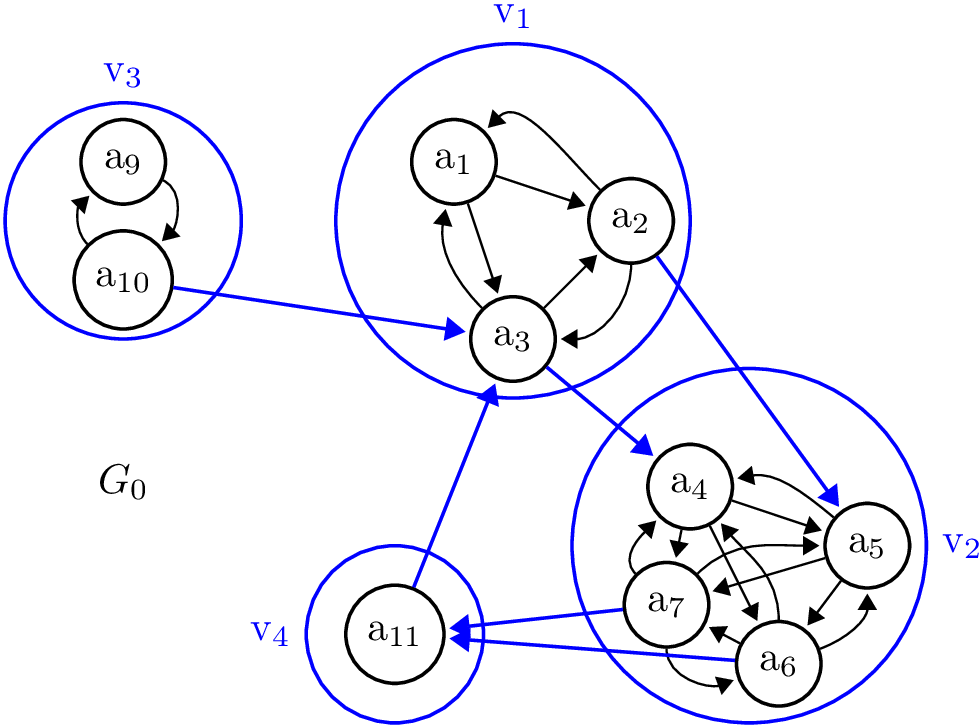
\includegraphics[scale=0.315]{Immagini/graph0.png}
    };

    \node[canvas is zy plane at x=5,draw,fill=white] at (0,0) {
        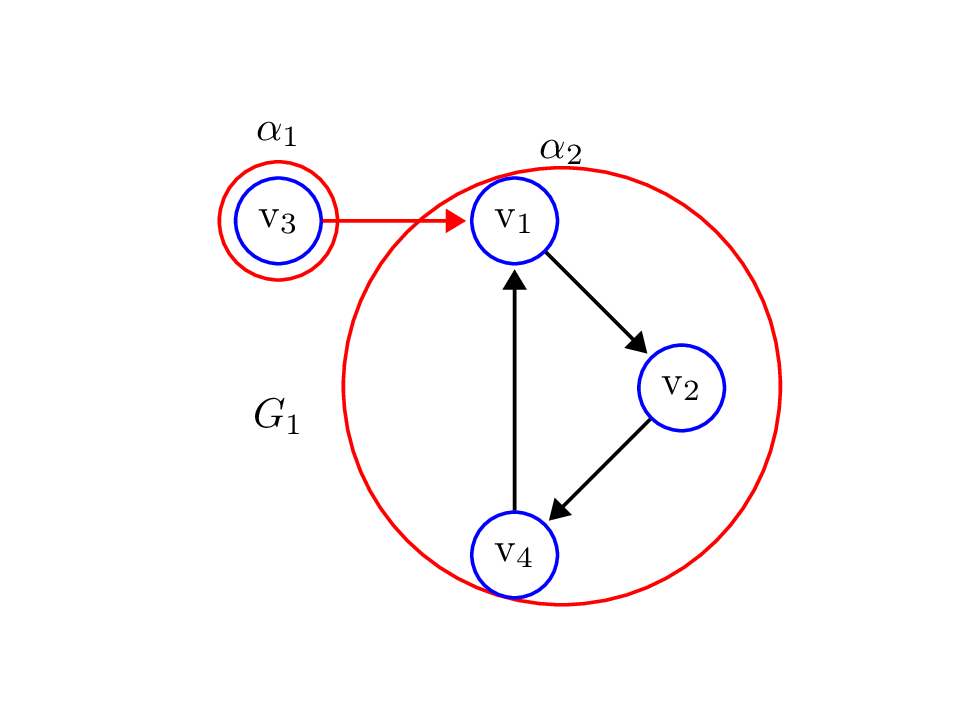
\includegraphics[scale=0.315]{Immagini/graph1.png}
    };

    \node[canvas is zy plane at x=10,draw,fill=white] at (0,0) {
        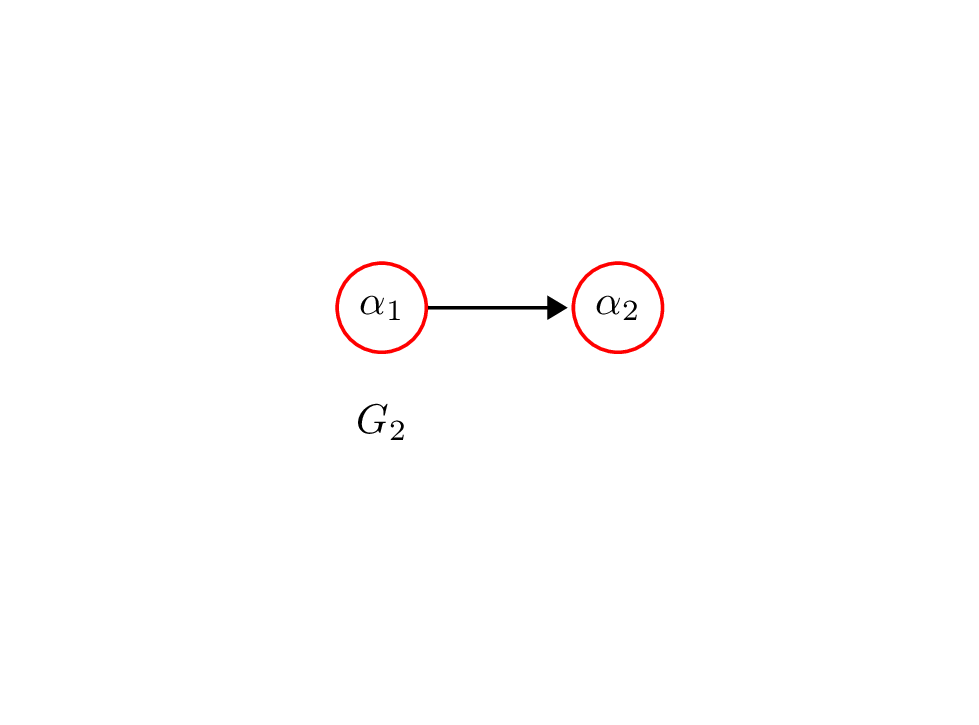
\includegraphics[scale=0.315]{Immagini/graph2.png}
    };
\end{tikzpicture}
        \caption{Esempio di grafo multilivello}
        \label{fig:multi-level-graph-example}
    \end{figure}

    \newpage

    \subsection{Algoritmo di trasformazione naturale}\label{subsec:algoritmo-di-trasformazione-naturale}

    La generica procedura algoritmica per realizzare la trasformazione naturale di un grafo standard $H = (W, F)$
    preso in input in un grafo decontraibile $G = (V, E)$, può essere definita considerando la creazione di supernodi
    e superarchi, costruendo implicitamente la funzione biiettiva $f_V: W \rightarrow V$ che realizza l'isomorfismo tra i nodi
    di $H$ e i supernodi di $G$.

    \begin{algorithm}[H] \floatname{algorithm}{Algoritmo}
    \begin{algorithmic}[1]
        \caption{NATURAL-TRANSFORMATION($H$)}\label{alg:natural-transformation}
        \State Sia $G = (V, E)$ un nuovo grafo decontraibile, con $V = \emptyset$ e $E = \emptyset$
        \For{$x \in W$}
            \State Sia $v$ un nuovo supernodo
            \State $v.dec \coloneqq (\emptyset, \emptyset)$
            \State $V \coloneqq V \cup \{v\}$
        \EndFor
        \For{$(x,y) \in F$}
            \State Sia $e$ un nuovo superarco
            \State $e.dec \coloneqq \emptyset$
            \State $E \coloneqq E \cup \{e\}$
        \EndFor
        \State \Return $G$
    \end{algorithmic}
\end{algorithm}

    Tramite l'ausilio di strutture dati con tempi di ricerca costanti, come insiemi di hash, la complessit\`a delle
    operazioni all'interno dei due circli \`e $O(1)$,
    e, di conseguenza, la complessit\`a dell'algoritmo \`e dettata dal numero di nodi e archi del grafo in input $H$,
    ovvero $\Theta(|W| + |F|)$.






\chapter{Algoritmi di enumerazione}

In informatica, un \textit{algoritmo di enumerazione} \`e un algoritmo che elenca tutte le possibili risposte ad un
problema computazionale in modo sistematico e completo. Tali algoritmi sono quindi progettati per ricevere un
determinato input, generare una lista esaustiva di tutte le possibili soluzioni senza duplicati e, solo allora,
terminare.
Quando si parla di algoritmi di enumerazione applicati al dominio dei grafi, allora spesso si intende il processo di
identificazione di sottoinsiemi di nodi o archi che soddisfano determinate caratteristiche.
In questo capitolo si tratteranno e analizzeranno alcuni utili algoritmi di enumerazione presenti in letteratura per
il riconoscimento di pattern strutturali all'interno di grafi. In particolare, si scuteranno algoritmi per l'enumerazione
di componenti fortemente connesse, di cricche e di circuiti semplici, problemi di notevole importanza nella teoria dei
grafi e ritenuti di interesse per la definizione di algoritmi di contrazione.
Questi algoritmi costituiranno il \"motore\" degli algoritmi presentati nei capitoli successivi, e saranno di
importanza fondamentale alla definizione degli algoritmi di contrazione usati per la costruzione di grafi multi-livello.

\section{Enumerazione di componenti fortemente connesse}\label{subsec:enumerazione-di-componenti-fortemente-connesse}
Come citato nel Capitolo 1, la condensazione di un grafo diretto \`e il suo grafo quoziente dove le componenti
fortemente connesse definiscono i blocchi della partizione.
Enumerare le componenti fortemente connesse di un grafo diretto $G = (V, E)$ significa trovare tutti i sottoinsiemi
che permettano di costruire una condensazione del grafo di partenza.
In questa sezione si discuter\`a un classico algoritmo di enumerazione delle componenti fortementi connesse, chiamato
da alcuni testi come l'algoritmo di Kosaraju~\cite{SHARIR198167} e al seguito si discuter\`a di un possibile adattamento
dell'algoritmo per la costruzione contestuale di un grafo contratto in forma di grafo decontraibile.

\subsection{Algoritmo di Kosaraju}\label{subsec:algoritmo-di-kosaraju}
L'algoritmo di Kosaraju (anche noto come algoritmo di Kosaraju-Sharir) \`e un algoritmo per l'enumerazione
delle componenti fortemente connesse di un grafo diretto dalla complessit\`a lineare scoperto nel 1978 da S. Rao
Kosaraju, ma pubblicato solamente nel 1981 da Micha Sharir, che lo scopri\`o indipendentemente.
Esso sfrutta il principio per cui le componenti fortemente connesse di un grafo diretto sono le stesse del suo grafo
trasposto, ovvero il grafo ottenuto invertendo l'orientamento di tutti gli archi.

A seguire alcune utili nozioni preliminari per la comprensione dell'algoritmo:

\paragraph{Grafo trasposto}
Dato un grafo diretto $G = (V, E)$, il suo grafo trasposto $G^T = (V, E^T)$ \`e il grafo ottenuto invertendo
l'orientamento di tutti gli archi di $G$, ovvero $E^T = \{(u, v) \mid (v, u) \in E\}$.
 \'E interessante notare che $G^T$ ha le stesse componenti fortemente connesse di $G$: se un cammino da $u$ a $v$
esiste in $G$, allora esiste anche un cammino da $v$ a $u$ in $G^T$.
Essendo le componenti fortemente connesse basate sulla mutua raggiungibilit\`a dei nodi, esse non cambiano
quando si invertono gli archi.

Una procedura algoritmica per il calcolo di $G^T$ non farebbe altro che scorrere linsieme di archi di $G$ e
invertirli, e sarebbe quindi di complessit\`a lineare.

\paragraph{Visita in profondit\`a}
La visita in profondit\`a di un grafo (in inglese \textit{depth-first search} o \textit{DFS}) \`e un particolare
algoritmo di visita che, in quanto tale, permette di visitare tutti i nodi di un grafo partendo da un nodo iniziale,
e di scoprire tutti i nodi raggiungibili da esso.
Ci\`o viene fatto in modo ricorsivo, visitando un nodo e poi applicando la procedura di visita ricorsivamente
a tutti i nodi ad esso adiacenti.
Nel corso dell'algoritmo i nodi vengono colorati in tre colori: bianco, grigio e nero, ad indicare rispettivamente
che il nodo non \`e stato visitato, che \`e in fase di visita e che \`e stato visitato.
Questo permette di non incorrere in cicli di visita infiniti nel caso non si stia visitando un grafo aciclico.
Nel corso dell'algoritmo vengono anche assegnati ai nodi due valori interi: il tempo di scoperta ($d$) e il tempo di
fine visita ($f$), che permettono di determinare, rispettivamente, l'ordine in cui i nodi vengono scoperti e il tempo
in cui la visita di un nodo termina.
Un attributo aggiuntivo, il predecessore, permette di memorizzare il nodo da cui si \`e scoperto il nodo corrente.

\paragraph{Ordinamento topologico}
Dato un grafo diretto aciclico $G = (V, E)$, un ordinamento topologico di $G$ \`e una particolare sequenza
dei suoi nodi $\langle v_1, v_2, \ldots, v_n \rangle$ tale che per ogni arco $(v_i, v_j) \in E$, $i < j$.
Si noti, quindi, che un ordinamento topologico di un grafo diretto pu\`o esistere solo se il grafo non contiene
cicli.
Una procedura algoritmica per il calcolo di un ordinamento topologico di $G$ pu\`o essere effettuata tramite una
visita in profondit\`a del grafo, raccogliendo in una lista concatenata i nodi in ordine decrescente di tempo
di fine visita, man mano che vengono visitati.
Per via del normale costo di una visita in profondit\`a, la complessit\`a di tale procedura \`e lineare.





La procedura segue la logica dell'algoritmo di Kosaraju per l'individuazione delle componenti strettamente connesse
descritto in [1], effettuando due visite in profondit\`a, una sul grafo originale $G$ e una sul grafo trasposto
$G^T$, in cui la seconda \`e effettuata secondo l'ordinamento topologico della prima.
Durante la seconda visita in profondit\`a viene costruito il grafo $G\mathcal{'}$ ottenuto come contrazione del
grafo decontraibile $G$.

    \begin{algorithm}[H]
    \caption{COMPONENT-CONTRACT($G$)}\label{alg:cap2}
    \begin{algorithmic}[1]
        \State call $DFS(G)$ to compute finishing times $u.f$ for each vertex $u$
        \State compute $G^T$
        \State $G\mathcal{'} = DFS\mathcal{'}(G^T)$ considering $G.V$ by finishing times in decreasing order
        \State \textbf{return} $G\mathcal{'} $
    \end{algorithmic}
\end{algorithm}

    Il seguente algoritmo descrive la seconda visita in profondit\`a, che include la costruzione del grafo
    contratto di $G$. \newline
    I parametri passati alla procedura ricorsiva DFS-VISIT' includono
    \begin{itemize}
        \item il grafo decontraibile originale  $G$
        \item il nodo da  visitare $u$
        \item il supernodo $\alpha_i$, che rappresenta una componente fortemente connessa di $G$ che include $u$
        \item i due insiemi da costruire $V_{\alpha_i}, E_{\alpha_i}$, che insieme definiscono il grafo $\alpha_i.dec = (V_{\alpha_i}, E_{\alpha_i})$ 
		associato al supernodo $\alpha_i$.
	    \item l'insieme di superarchi $\mathfrak{E}$, che vengono definiti nel corso della visita.
		Gli archi in $\epsilon.dec$ con $\epsilon \in \mathfrak{E}$ vengono aggiunti quando si incontrano nodi appartenenti
        ad altre componenti connesse gi\`a visitate.
    \end{itemize}

    \begin{algorithm}[!H]
    \caption{DFS$\mathcal{'}$($G$)}\label{alg:cap3}
    \begin{algorithmic}[1]
        \For {each $v \in G.V$}
            \State $v.color =$ WHITE
        \EndFor
        \State $\mathfrak{V} \coloneqq \emptyset$
        \State $\mathfrak{E} \coloneqq \emptyset$
        \State i $\coloneqq$ 0
        \For {each $u \in G.V$ in decreasing order by $u.f$}
            \If {$u.color ==$ WHITE}
                \State let $\alpha$ be a new super-node
                \State $\mathfrak{V} \coloneqq \mathfrak{V} \cup \{\alpha_i\}$
                \State $V_{\alpha_i} \coloneqq \emptyset$
                \State $E_{\alpha_i} \coloneqq \emptyset$
                \State DFS-VISIT'($G, u, \alpha, V_{\alpha_i}, E_{\alpha_i}, \mathfrak{E}$)
                \State $\alpha.dec \coloneqq$ $(V_{\alpha_i}, E_{\alpha_i})$
                \State $i \coloneqq i + 1$
            \EndIf
        \EndFor
        \State $G\mathcal{'} \coloneqq (\mathfrak{V}, \mathfrak{E})$
        \State \textbf{return} $G\mathcal{'}$
    \end{algorithmic}
\end{algorithm}
    \begin{algorithm}[!H]
    \caption{DFS-VISIT'($G, u, \alpha, V_{\alpha}, E_{\alpha}, \mathfrak{E}$)}\label{alg:cap}
    \begin{algorithmic}[1]
        \State $u.color \coloneqq$ GREY
        \State $u.supernode \coloneqq \alpha$
        \State $V_{\alpha} \coloneqq V_{\alpha} \cup \{u\}$
        \For {each $v \in G.adj[u]$}
            \If {($v.color ==$ WHITE $\vee$ $v.supernode == \alpha$)}
                \State $E_{\alpha} \coloneqq E_{\alpha} \cup  (v ,u)$
            \EndIf
            \If{($v.color ==$ WHITE)}
                \State DFS-VISIT'($G, v, \alpha, V_{\alpha}, E_{\alpha}, \mathfrak{E}$)
            \ElsIf{($v.color ==$ BLACK $\wedge$ $v.supernode \ne \alpha$)}
            \If{$(v.supernode, \alpha) \notin \mathfrak{E}$}
                \State $(v.supernode, \alpha).dec \coloneqq \emptyset$
                \State $\mathfrak{E} \coloneqq \mathfrak{E} \cup \{(v.supernode, \alpha)\}$
            \EndIf
            \State $(v.supernode, \alpha).dec \coloneqq (v.supernode, \alpha).dec \cup \{(v, u)\}$
            \EndIf
        \EndFor
        \State $u.color \coloneqq$ BLACK
    \end{algorithmic}
\end{algorithm}

    \newpage

    \begin{figure}
        \resizebox{!}{3.3cm}{
            \begin{tikzpicture}
                %comp 1
                \node[mynode](n1) at (0,0){1};
                \node[mynode](n2) at (1.2,-1){2};
                \node[mynode](n3) at (1.2, 1){4};
                \node[mynode](n4) at (2.4, 0){3};
                \draw[myarrow](n1)--(n2);
                \draw[myarrow](n3)--(n1);
                \draw[myarrow](n4)--(n3);
                \draw[myarrow](n2)--(n4);
                %comp 2
                \node[mynode](n5) at (4,1.2){5};
                \node[mynode](n6) at (4,0){6};
                \node[mynode](n7) at (4, -1.2){7};
                \draw[myarrow](n6) -- (n5);
                \draw[myarrow](n5) to[out=3,in=3] (n7);
                \draw[myarrow](n7) -- (n6);

                %comp edges
                \draw[myarrow](n3) -- (n5);
                \draw[myarrow](n2) -- (n7);
                %comp 3
                \node[mynode](n8) at (6, 2){8};
                %comp 4
                \node[mynode](n9) at (8, 2){9};
                \node[mynode](na) at (8.5, 0){10};
                \draw[myarrow](n9) -- (n8);
                \draw[myarrow](na) to[out=3,in=3] (n9);
                \draw[myarrow](n9) -- (na);
                \draw[myarrow](n8) -- (n5);

                \node[below=10mm] at (5, -1.2) {(a)};
            \end{tikzpicture}
            \begin{tikzpicture}
                %comp 1
                \node[mynode, label=above:{$13/20$}, fill=black](n1) at (0,0){\textcolor{white}{1}};
                \node[mynode, label=above:{$14/19$}, fill=black](n2) at (1.2,-1){\textcolor{white}{2}};
                \node[mynode, label=above:{$16/17$}, fill=black](n3) at (1.2, 1){\textcolor{white}{4}};
                \node[mynode, label=above:{$15/18$}, fill=black](n4) at (2.4, 0){\textcolor{white}{3}};
                \draw[myarrow](n1)--(n2);
                \draw[myarrow](n3)--(n1);
                \draw[myarrow](n4)--(n3);
                \draw[myarrow](n2)--(n4);
                %comp 2
                \node[mynode, label=above:{$5/10$}, fill=black](n5) at (4,1.2){\textcolor{white}{5}};
                \node[mynode, label=right:{$7/8$}, fill=black](n6) at (4,0){\textcolor{white}{6}};
                \node[mynode, label=below:{$6/9$}, fill=black](n7) at (4, -1.2){\textcolor{white}{7}};
                \draw[myarrow](n6) -- (n5);
                \draw[myarrow](n5) to[out=3,in=3] (n7);
                \draw[myarrow](n7) -- (n6);

                %comp edges
                \draw[myarrow](n3) -- (n5);
                \draw[myarrow](n2) -- (n7);
                %comp 3
                \node[mynode, label=above:{$4/11$}, fill=black](n8) at (6, 2){\textcolor{white}{8}};
                %comp 4
                \node[mynode, label=above:{$1/12$}, fill=black](n9) at (8, 2){\textcolor{white}{9}};
                \node[mynode, label=below:{$2/3$}, fill=black](na) at (8.5, 0){\textcolor{white}{10}};
                \draw[myarrow](n9) -- (n8);
                \draw[myarrow](na) to[out=3,in=3] (n9);
                \draw[myarrow](n9) -- (na);
                \draw[myarrow](n8) -- (n5);

                % label for the second graph
                \node[align=center, xshift=0.5cm, yshift=2.3cm] (label2) {$\langle 1, 2, 3, 4, 9, 8, 5, 7, 6, 10 \rangle$};
                \node[below=10mm] at (5, -1.2) {(b)};
            \end{tikzpicture}
            \label{fig:alg1}}
    \end{figure}

    \begin{figure}
        \resizebox{!}{3.9cm}{
            \begin{tikzpicture}
                %comp 1
                \node[mynode](n1) at (0,0){1};
                \node[mynode](n2) at (1.2,-1){2};
                \node[mynode](n4) at (1.2, 1){4};
                \node[mynode](n3) at (2.4, 0){3};
                \draw[myarrow](n2)--(n1);
                \draw[myarrow](n1)--(n4);
                \draw[myarrow](n4)--(n3);
                \draw[myarrow](n3)--(n2);
                %comp 2
                \node[mynode](n5) at (4,1.2){5};
                \node[mynode](n6) at (4,0){6};
                \node[mynode](n7) at (4, -1.2){7};
                \draw[myarrow](n5) -- (n6);
                \draw[myarrow](n7) to[out=3,in=3] (n5);
                \draw[myarrow](n6) -- (n7);

                %comp edges
                \draw[myarrow](n5) -- (n4);
                \draw[myarrow](n7) -- (n2);
                %comp 3
                \node[mynode](n8) at (6, 2){8};
                %comp 4
                \node[mynode](n9) at (8, 2){9};
                \node[mynode](na) at (8.5, 0){10};
                \draw[myarrow](n8) -- (n9);
                \draw[myarrow](n9) to[out=3,in=3] (na);
                \draw[myarrow](na) -- (n9);
                \draw[myarrow](n5) -- (n8);

                \node[align=center, xshift=0.5cm, yshift=2.3cm] (label2) {$\langle 1, 2, 3, 4, 9, 8, 5, 7, 6, 10 \rangle$};
                \node[below=10mm] at (5, -1.2) {(c)};
            \end{tikzpicture}
            \begin{tikzpicture}
                %comp 1
                \node[mynode, fill={rgb:red,4;green,2;yellow,1}](n1) at (0,0){\textcolor{white}{1}};
                \node[mynode, fill={rgb:red,4;green,2;yellow,1}](n2) at (1.2,-1){\textcolor{white}{2}};
                \node[mynode, fill={rgb:red,4;green,2;yellow,1}](n4) at (1.2, 1){\textcolor{white}{4}};
                \node[mynode, fill={rgb:red,4;green,2;yellow,1}](n3) at (2.4, 0){\textcolor{white}{3}};
                \draw[myarrow, color={rgb:red,4;green,2;yellow,1}](n2)--(n1);
                \draw[myarrow, color={rgb:red,4;green,2;yellow,1}](n1)--(n4);
                \draw[myarrow, color={rgb:red,4;green,2;yellow,1}](n4)--(n3);
                \draw[myarrow, color={rgb:red,4;green,2;yellow,1}](n3)--(n2);
                %comp 2
                \node[mynode, fill=red](n5) at (4,1.2){\textcolor{white}{5}};
                \node[mynode, fill=red](n6) at (4,0){\textcolor{white}{6}};
                \node[mynode, fill=red](n7) at (4, -1.2){\textcolor{white}{7}};
                \draw[myarrow, red](n5) -- (n6);
                \draw[myarrow, red](n7) to[out=3,in=3] (n5);
                \draw[myarrow, red](n6) -- (n7);
                %comp edges
                \draw[myarrow, color={rgb:red,1;blue,2}](n5) -- (n4);
                \draw[myarrow, color={rgb:red,1;blue,2}](n7) -- (n2);
                %comp 3
                \node[mynode, fill=green!50!red](n8) at (6, 2){\textcolor{white}{8}};
                %comp 4
                \node[mynode, fill={rgb:red,1;green,2;blue,5}](n9) at (8, 2){\textcolor{white}{9}};
                \node[mynode, fill={rgb:red,1;green,2;blue,5}](na) at (8.5, 0){\textcolor{white}{10}};
                \draw[myarrow, color={rgb:red,4;green,1;blue,3}](n8) -- (n9);
                \draw[myarrow, color={rgb:red,1;green,2;blue,5}](n9) to[out=3,in=3] (na);
                \draw[myarrow, color={rgb:red,1;green,2;blue,5}](na) -- (n9);
                \draw[myarrow, color={rgb:red,2;green,1}](n5) -- (n8);

                \node[align=center, xshift=0.5cm, yshift=2.3cm] (label2) {$\langle \rangle$};

                \begin{scope}[shift={(0,-3.2)}]
                \node[mynode,
                    label={[align=center]above:{$V_{1\mathcal{'}} = \{1, 4, 3, 2\}$}\\{\tiny$E_{1\mathcal{'}} = \{(4,1), (3, 4), (2, 3), (1, 2)\}$}},
                    fill={rgb:red,4;green,2;yellow,1}](n1) at (0, 0){\textcolor{white}{$1\mathcal{'}$}};
                \node[mynode,
                    label={[align=center]above:{$V_{4\mathcal{'}} = \{5, 6, 7\}$}\\{\tiny$E_{4\mathcal{'}} = \{(6, 5), (7, 6), (5, 7)\}$}},
                    fill=red](n4) at (3.5, 0){\textcolor{white}{$4\mathcal{'}$}};
                \node[mynode,
                    label={[align=center]above:{$V_{3\mathcal{'}} = \{8\}$}\\{\tiny$E_{3\mathcal{'}} = \{\}$}},
                    fill=green!50!red](n3) at (6.5, 0){\textcolor{white}{$3\mathcal{'}$}};
                \node[mynode,
                    label={[align=center]above:{$V_{2\mathcal{'}} = \{9, 10\}$}\\{\tiny$E_{2\mathcal{'}} = \{(10,9), (9, 10)\}$}},
                    fill={rgb:red,1;green,2;blue,5}](n2) at (9, 0){\textcolor{white}{$2\mathcal{'}$}};

                \draw[myarrow,
                    color={rgb:red,4;green,1;blue,3}](n2) to node [below]{\tiny$E_{e_1} = \{(9, 8)\}$} (n3);
                \draw[myarrow,
                    color={rgb:red,1;blue,2}](n1) to node [below]{\tiny$E_{e_2} = \{(4, 5), (2, 7)\}$} (n4);
                \draw[myarrow,
                    color={rgb:red,2;green,1}](n3) to node [below]{\tiny$E_{e_3} = \{(8, 5)\}$} (n4);

                \node[below=10mm] at (5, 0) {(d)};
                \end{scope}
            \end{tikzpicture}
            \label{fig:alg2}}
        \caption{Rappresentazione delle fasi rilevanti dell'algoritmo COMPONENT-CONTRACTION applicato al grafo in (a).
        In (b) \`e rappresentato lo stato del grafo al termine della procedura DFS, assieme alla lista dei nodi ordinata
        per tempi di fine visita (ordinamento topologico). In (c) il grafo trasposto ottenuto invertendo gli archi del
        grafo in (a). In (d) lo stato del grafo trasposto in (c) al termine della procedura DFS$\mathcal{'}$, assieme al grafo
        contratto costruito.}
    \end{figure}

    \newpage
    In particolare:
    \begin{itemize}
        \item i nodi $v$ che soddisfano la condizione a riga 5 di DFS-VISIT$\mathcal{'}$ fanno parte della stessa componente di $u$.
        Per questi nodi l'arco originale del grafo non trasposto $(v, u)$ viene aggiunto al grafo corrispondente al
        supernodo $\alpha$ a riga 6;
        \item i nodi $v$ che soddisfano la condizione a riga 10 di DFS-VISIT$\mathcal{'}$ sono nodi che fanno parte di altre
        componenti fortemente connesse gi\`a visitate che sono adiacenti a $u$.
        Per questi nodi, si considerano i superarchi ottenuti dai rispettivi supernodi di $v$ e $u$, aggingendoli a
	    $\mathfrak{E}$ se necessario, (riga 13), e aggiungendo l'arco originale $(v, u)$ all'insieme di archi
        rappresentato dal superarco (riga 15).
    \end{itemize}

    \paragraph{Complessit\`a dell'algoritmo}
    L'algoritmo COMPONENT-CONTRACT applicato ad un grafo $G = (V, E)$  mantiene una complessit\`a temporale di
    $\Theta(V + E)$, in quanto:
    \begin{itemize}
        \item A riga 1 viene eseguita una ricerca in profondit\`a tradizionale, quindi con costo $\Theta(V + E)$.
        \item A riga 2 viene costruito il grafo trasposto $G^T = (V, E^T)$, dove $E^T = \{(u, v) \mid (v, u) \in E\}$ \`e
        dato dagli archi in $E$ con orientamento invertito.
        Anche in questo caso, la sua costruzione pu\`o avvenire in un tempo $O(V + E)$, iterando prima sull'insieme dei
        nodi di $G$ e poi sui suoi archi, invertendone l'orientamento.
        L'ordinamento dei nodi di $G^T$ pu\`o essere realizzato nel corso della visita a riga 1 attraverso la costruizione
        di una lista concatenata, per cui i nodi possono essere aggiunti in testa alla lista in tempo $O(1)$  man mano
        che viene loro assegnata l'etichetta di fine visita $u.f$.
        \item A riga 3 viene eseguita la procedura DFS' che corrisponde ad una visita in profondit\`a di $G^T$ abbinata
        alle operazioni di costruzione del grafo decontraibile.
        In particolare, le operazioni che vengono effettuate in aggiunta a quelle di una visita in profondit\`a consistono
        nei semplici assegnamenti alle righe 4\textendash6, 10\textendash12, 14\textendash15 e 18 di DFS' e alle righe
        2\textendash3 di DFS-VISIT'.
        Inoltre sono previsti dei controlli e dei relativi assegnamenti alle righe 5\textendash7 e 10\textendash16 che,
        ancora una volta, aggiungono solamente costi costanti per ogni arco in $G^T$.
        Il costo computazionale della procedura rimane $\Theta(V + E)$.
    \end{itemize}

    \subsection{Correttezza dell'algoritmo}\label{subsec:correttezza-dell'algoritmo}

    \paragraph{Lemma 3.2.1}
    Sia $G=(V,E)$ un grafo decontraibile input dell'algoritmo COMPONENT-CONTRACT, sia $G\mathcal{'}$ il grafo decontraibile
    in output, sia $u$ un nodo in $V$, sia $v$ un nodo adiacente a $u$ in $(G)^T$, sia $\alpha$ il supernodo di $u$.
    Le condizioni sul nodo $v$ alle righe 5 e 10 di DFS-VISIT' sono tra loro mutualmente esclusive e ricoprono tutti i
    possibili casi.
    In particolare:
    \begin{enumerate}[(i)]
        \item ($v.color ==$ WHITE $\vee$ $v.supernode == \alpha$) $\implies$ il nodo $v$ ha lo stesso supernodo di $u$ al
        termine dell'algoritmo.
        \item ($v.color ==$ BLACK $\wedge$ $v.supernode \ne \alpha$) $\implies$ il nodo $v$ non ha lo stesso supernodo di
        $u$ al termine dell'algoritmo.
    \end{enumerate}

    \paragraph{Dimostrazione}
    Si noti, innanzitutto, che l'attributo $supernode$ una volta assegnato non viene pi\`u modificato fino al termine
    dell'algoritmo, in quanto esso pu\`o essere assegnato solamente a riga 2 di DFS-VISIT' e DFS-VISIT' viene richiamato
    una ed una sola volta per ciascun nodo. \newline

    Per dimostrare (i) ci limitiamo a dimostrare $v.color ==$ WHITE $ \implies v.supernode == u.supernode$ e
    $v.supernode == \alpha \implies v.supernode == u.supernode$.
    \begin{enumerate}
        \item Assumiamo $v.color ==$ WHITE. Questo significa che esso non ha ancora alcun supernodo assegnato e che gli 
		verr\`a assegnato il supernodo $\alpha$ nella chiamata di DFS-VISIT' a riga 9, in quanto la condizione a riga 8
        \`e verificata $(H_1)$.
        \item Assumiamo $v.supernode == \alpha$.
        Banalmente, essendo $u.supernode = \alpha$ si ottiene $v.supernode == u.supernode$ $(H_2)$.
    \end{enumerate}
    Per $(H_1)$ e $(H_2)$ abbiamo dimostrato il punto (i).

    Per dimostrare (ii) assumiamo $v.color ==$ BLACK $(H_3)$ e $v.supernode \ne \alpha$ $(H_4)$.
    Dato $(H_3)$, il nodo $v$ \`e gi\`a stato visitato e deve, pertanto, avere un supernodo assegnato.
    Per $(H_4)$, questo supernodo non pu\`o essere $\alpha = u.supernode$, pertanto si conclude
    $v.supernode \neq u.supernode$. \newline

    Le conclusioni dei punti (i) e (ii) risultano essere, quindi, mutualmente esclusive e ricoprono tutti i possibili
    casi sullo stato del nodo $v$ ed $u$ al termine dell'algoritmo.

    \paragraph{Correttezza dell'algoritmo}
    Al termine dell'esecuzione dell'algoritmo su un grafo decontraibile $G\coloneqq(V, E)$ avremo costruito un grafo
    decontraibile $G\mathcal{'} \coloneqq (\mathfrak{V}, \mathfrak{E})$ dove:
    \begin{enumerate}[(i)]
        \item $G\mathcal{'}$ \`e una contrazione di $G$
        \item Per ogni supernodo $\alpha \in \mathfrak{V}$, con $\alpha.dec = (V_{\alpha}, E_{\alpha})$, $V_{\alpha}$ \`e una componente fortemente
        connessa di $G$
    \end{enumerate}

    \paragraph{Dimostrazione}
    La propriet\`a (i) pu\`o essere dimostrata notando che:
    \begin{itemize}
        \item La prima propriet\`a delle contrazioni \`e rispettata, in quanto ogni nodo $u \in V$ viene visitato una ed una
        sola volta da DFS-VISIT' e viene aggiunto ad un certo insieme $V_{\alpha}$ per qualche $\alpha \in \mathfrak{V}$.
        Inoltre, per ogni supernodo $\alpha \in \mathfrak{V}$, $V_{\alpha} \neq \emptyset$ in quanto esso dovr\`a contenere
        almeno il nodo $u$ della prima chiamata di DFS-VISIT' a riga 13 di DFS'.

        \item La seconda propriet\`a delle contrazioni \`e rispettata.
        Per il Lemma 3.2.1 le condizioni sul nodo $v$ alle righe 5 e 10 di DFS-VISIT' sono tra loro mutualmente
        esclusive e ricoprono tutti i possibili casi al termine dell'algoritmo: o $v$ ha lo stesso supernodo di $u$ o
        non ha lo stesso supernodo di $u$.
        Quindi si pu\`o notare che tutti gli archi in $E$ sono considerati ognuno una ed una sola volta dal ciclo for a
        riga 4 di DFS-VISIT'. Per ognuno di questi archi $(v, u)$, o vengono aggiunti ad un certo insieme $E_{\alpha}$
        per qualche $\alpha$ quando $u$ e $v$ sono tali per cui $u.supernode = v.supernode = \alpha$, o vengono aggiunti ad
        un insieme $e.dec$ per qualche $e \in \mathfrak{E}$ quando $u$ e $v$ sono tali per cui
        $u.supernode \neq v.supernode$.
        Questo vuol dire che
        $\{ E_\alpha \mid \alpha \in \mathfrak{V}$, $\alpha.dec = (V_\alpha, E_\alpha)\} \cup \{ \epsilon .dec \mid \epsilon \in \mathfrak{E}\}$
        \`e un ricoprimento di $E$ formato di insiemi a due a due disgiunti. \newline
        Inoltre, la propriet\`a per cui $\emptyset \notin \{\epsilon .dec \mid \epsilon \in \mathfrak{E}\}$ \`e garantita dal fatto che
        l'esecuzione della riga 13 di DFS-VISIT' \`e sempre succeduta dall'esecuzione della riga 16, per cui non pu\`o
        esistere $\epsilon \in \mathfrak{E}$ tale per cui $\epsilon .dec = \emptyset$.
    \end{itemize}

    La propriet\`a (ii) pu\`o essere dimostrata notando che l'agoritmo utilizza la stessa logica dell'algoritmo per
    l'individuazione delle componenti connesse descritto in [1].
    In particolare, \`e possibile dimostrare per induzione che alla k-esima chiamata di DFS-VISIT', le componenti
    connesse $C_i$ con $ i = 0,\ldots, k-1$, tali per cui $f(C_i)$ \`e il tempo di fine visita massimo tra i nodi della
    componente i-esima e, quindi, tali per cui $f(C_i) > f(C_k)$ $\forall i$, sono state gi\`a visitate e assegnate a
    degli insiemi $V_{\alpha_i}$ per dei supernodi $\alpha_i$.
    Inoltre, per il Lemma 22.15 descritto in [1], le componenti $C'$ tali per cui $f(C') < f(C_k)$ non possono essere
    visitate durante la visita dell'albero di $C_k$, in quanto in $G^T$ non possono esistere archi della forma $(v ,u)$
    con $v \in C' $ e $ u \in C_k$.
    Per l'assegnamento a riga 3 di DFS-VISIT', ogni nodo visitato viene aggiunto all'insieme $V_{\alpha_i}$, il quale cambia
    a riga 11 di DFS' per ogni nuovo albero di ricerca in profondit\`a che viene percorso.
    Pertanto al termine dell'algoritmo $V_{\alpha_i}$ rappresenter\`a una componente fortemente connessa di $G$ per ogni $\alpha_i$.

\chapter{Applicazioni dei Grafi Multilivello}

\subsection{Possibili applicazioni della contrazione}
Nel contesto generale dell'analisi di grafi, la contrazione di nodi e archi pu\`o essere utile per:
\begin{itemize}
    \item Ridurre la complessit\`a dell'analisi strutturale di un grafo, sia che esso debba essere processato
    attraverso algoritmi costosi, sia che esso debba essere graficamente visualizzato, rendendolo pi\`u facilmente
    interpretabile ed evidenziando le caratteristiche strutturali di interesse.
    \item Studiare l'interrelazione di caratteristiche strutturali di un grafo, che rappresenti la navigabilit\`a
    di uno spazio basato su componenti fortemente connesse, cicli, cricche ecc.
    \item Stabilire il grado di connettivit\`a di un grafo, individuando la rilevanza (intesa come il numero di
    insiemi componente che rappresentano i supernodi), il numero e la dimensione delle sue contrazioni.
    \item Misurare il grado di complessit\`a dello spazio rappresentativo del grafo, in base al numero
    di nodi e archi presenti nelle contrazioni (grafi derivanti da specifici domini tendono ad avere un certo grado
    di complessit\`a legato ad un concetto spaziale).
    \item Valutare l'influenza di singoli nodi e archi sulla struttura contratta del grafo, eseguendo analisi
    della sensitivit\`a e della robustezza del grafo.
\end{itemize}

Nel contesto dell'analisi di testi in linguaggio naturale, in particolare di sogni, e della loro rappresentazione
tramite grafi, con l'ausilio di strumenti di analisi NLP per un eventuale preprocessing, la contrazione di
nodi essere utile per:
\begin{itemize}
    \item Individuare contesti sintattici (e possibilmente semantici) di parole e frasi, evidenziando l'interrelazione
    e la distanza tra gruppi di parole e frasi.
    \item Valutare la somiglianza di singoli brevi testi, come il racconto dei sogni, individuando le
    macro-caratteristiche strutturali comuni e le differenze tra esse.
    \item Individuare pattern ricorrenti di parole e insiemi di parole su un corpus pi\`u ampio di testi, con
    eventuale ausilio di strumenti statistici.
    \item Stabilire il grado di connettivit\`a del grafo delle parole in base al numero di insiemi componente
    (gruppi di parole) e di nodi presenti nelle contrazioni.
    \item Permettere un confronto automatico dei pattern strutturali con grafi multilivello che rappresentino
    un controllo, con l'eventuale ausilio di algoritmi che valutano il grado di somiglianza di grafi.
\end{itemize}

%\chapter{Conclusioni e Sviluppi Futuri}
\label{chap:conc}


 


\appendix
%\input{schema_elettrico}
%\input{Appendix1}
%\input{Appendix2}

% Citazioni nel testo
~\nocite{*} % Include tutte le voci nel .bib, anche se non citate nel testo
% Stampa la bibliografia
\printbibliography

\printindex

%\chapter*{Ringraziamenti}

Ringrazio...

\end{document}